\chapter{Introducci\'on}



\section{Estructura de este trabajo}

Este primer capítulo introductorio está dividido en dos secciones que presentan los aspectos necesarios para comprender el trabajo realizado, el cual se centra en el diseño de nuevas secuencias linkers 
siguiendo los requerimientos de diseño que se 
% con propiedades conformacionales definidas, restringiendo cualquier actividad biológica y elemento estructural no deseado.
En la primer sección (\ref{proteinLandscape}) se describe el amplio panorama conformacional y funcional que pueden presentar las proteinas, lo que da una idea de cuales son las elementos proteicos que pueden encontrarse.
% identificando cuáles son los elementos funcionales que pueden de acuerdo a las propiedades estructurales que adquieren.
% in-vivo, describiendo cuales son los posibles destinos de las proteinas desde que son sintetizadas en el ribosoma y a lo largo de su etapa funcional en la célula. 
% Se desarrollan los conocimientos actuales acerce del perfil de conformaciones y funciones conocidas, y las propiedades secuenciales asociadas con estas.
% Se intenta describir como estos conocimientos actuales sobre las propiedades conformacionales y funcionales de las proteinas se trasladan en el desarrollo 
% de un amplio abanico de metodos y herramientas bioinformaticas que, a su vez, permiten nuevos avances en los conocimientos subyacentes.
En la sección siguiente (\ref{proteinEngineering}) se desarrolla el tema de ingeniería de proteínas quiméricas, introduciendo el problema de cómo y por qué diseñar nuevas secuencias linker.

En el capítulo \ref{method} se describe la implementación desarrollada para el diseño de secuencias linker, indicando los fundamentos y detalles del método.
% , limitaciones y aspectos relevantes de su utilización.

En el capítulo \ref{tools} se detalla los distintos recursos utilizados para evaluar las propiedades de interés sobre la secuencia, describiendo el objetivo de cada evaluación y los fundamentos de cada método. 

En el capítulo \ref{manual} se documentan todos los aspectos necesarios para poder hacer uso de la herramienta.

En el capítulo \ref{results} se muestran, en primer lugar, las evaluaciones realizadas para obtener los parámetros óptimos de ejecución. 
Además, se evalúan distintas propiedades de la herramienta resultante y su ejecución analizando, luego, las secuencias obtenidas. 

Finalmente, el capítulo \ref{conclusiones} contiene las discusiones relevantes, conclusiones y trabajo a futuro.






\section{Módulos en proteínas}
\label{proteinLandscape}
%     1.2.1. Definición de proteína (1 página, 1 figura)
%     1.2.2. Estructura modular de las proteínas (1 página, de las páginas 28-29, 1 figura)
%     1.2.3. Módulos proteicos: estructuras, secuencias y funciones (14 páginas)
%         1.2.3.1. Proteínas globulares (4 páginas, 3 figuras)
%             1.2.3.1.1. Estructura de las proteínas globulares (secundaria, terciaria, cuaternaria)
%             1.2.3.1.2. Secuencias de las proteínas globulares
%             1.2.3.1.3. Actividades de las proteínas globulares
%         1.2.3.2. Proteínas de membrana (2 páginas, 1 figura)
%             1.2.3.2.1. Estructura de las proteínas de membrana (secundaria, terciaria, cuaternaria)
%             1.2.3.2.2. Secuencias de las proteínas de membrana
%             1.2.3.2.3. Actividades de las proteínas de membrana
%         1.2.3.3. Proteínas intrínsecamente desordenadas (4 páginas, 3 figuras)
%             1.2.3.3.1. Estructura de las proteínas intrínsecamente desordenadas
%             1.2.3.3.2. Secuencias de las proteínas intrínsecamente desordenadas
%             1.2.3.3.3. Actividades de las proteínas intrínsecamente desordenadas
%         1.2.3.4. Agregados proteicos (fibras amiloides, agregados amorfos, priones...) (3 páginas, 2 figuras)
%            1.2.3.4.1. Estructura de los agregados proteicos
%            1.2.3.4.2. Secuencias de los agregados proteicos
%            1.2.3.4.3. Actividades de los agregados proteicos
%         1.2.3.5. Comentario a las clasificaciones de los módulos: el continuo de estructuras, secuencias y actividades (1 página, 1 figura)
% 

\subsection{Definición inicial de una proteína}
Las proteínas son polímeros de aminoácidos y como tales, sus propiedades conformaciones y funcionales estan asociadas a la secuencia especifica que la define, 
Es decir, las diferentes combinaciones de aminoacidos les asignan distintas capacidades de interacción intramoleculares y con el contexto en el que se encuentra.
% La proteina queda definida por esta secuencia especifica la cual define las posibles interacciones, entre los residuos de la cadena o con el contexto en el que se encuentra. 
% De esta forma, la secuencia específica que compone una proteína define las propiedades conformacionales resultantes y las posibles funciones asociadas a esta.
% y las posibles funciones que puede desarrollar la proteína.
% La cadena polipeptídica puede formar interacciones que involucren a la estructura intrínseca del polipeptido(cadena carbonada y función amino) 
% e interacciones que involucren a la cadena lateral de los distintos aminoácidos, 
La diversidad de aminoácidos existentes permite una gran cantidad de combinaciones, lo que resulta en un perfil de propiedades conformacionales y funcionales muy amplio.

Por definición, una proteína puede estar compuesta por cadenas lineales formadas por cualquier combinación de aminoácidos.
Sin embargo, las proteínas se originan en la naturaleza como producto de los sistemas biológicos, por lo tanto, 
la ocurrencia de las proteínas naturales no se origina por cadenas peptídicas generadas al azar. 
Por el contrario, la ocurrencia de proteínas está ajustada a los requerimientos del sistema y al mecanismo evolutivo subyacente. 
Por lo tanto, el resultado es conjunto de proteínas con un perfil complejo donde cada una tendrá características únicas que determinan su actividad biológica dentro del sistema.
Basándose en estas condiciones, las proteínas naturales quedan mejor definidas si se describen las propiedades secuenciales, estructurales y las actividades biológicas asociadas. 

Cada proteína, entonces, quedará definida por el conjunto de propiedades que la describen, no sólo como polímero(secuencia de aminoácidos) 
sino también como módulo del sistema biológico (perfil de conformaciones en el contexto celular/sistémico, funcionalidades, interacciones, adaptaciones a cambios en el entorno, etc). 

Si bien cada proteína tendrá algunas propiedades individuales únicas(por ejemplo la secuencia de AAs), 
% el perfil de actividades realizadas por las proteínas no es tan complejo y 
el conjunto de proteínas naturales puede clasificarse 
agrupándolas de acuerdo a propiedades secuenciales y conformacionales, donde cada clase está asociada a cierto perfil de actividades biológicas que se derivan de estas propiedades.
En las próximas secciones de este capítulo, cuando se describan alguno de los elementos proteícos naturales, 
se detallarán las propiedades secuenciales y conformacionales asociadas y el perfil de actividades biológicas que realizan.









\subsection{Estructura modular de las proteínas}

Las proteínas naturales son usualmente modulares, conteniendo regiones definidas asociadas cada una con una subfunción específica.
Esta naturaleza modular provee muchas ventajas, principalmente la posibilidad de desarrollar funciones que requieren cooperación de distintos módulos, y un incremento en la estabilidad de la estructura global.
Otra ventajas incluyen la protección de los metabolitos intermedios dentro de espacios inter-dominio, aumentando la eficiencia global y previniendo la liberación al medio de intermediarios inestables de la reacción.  
Desde el punto de vista evolutivo, la modularidad en las proteínas incrementa la capacidad evolutiva reduciendo las restricciones necesarias 
para la adaptación y permitiendo que módulos preexistentes puedan funcionar en nuevos contextos para nuevos usos.

El módulo o unidad de proteína más común es el dominio, el cual puede adquirir distintas definiciones según las propiedades que se analicen:
Podemos definir a un dominio como una unidad evolutiva independiente que puede dar una proteína mono-dominio o formar parte de una multi-dominio. 
Cada unidad(dominio) puede tener una función independiente o contribuir a la función global de una proteína multi-dominio cooperando con el resto de las unidades.
Esta definición de dominio como unidad evolutiva es la que se usa como mecanismo de clasificación en la base de datos SCOP(Structural Classification of Proteins)\cite{murzin1995scop}. 

A diferencia de esto, en CATH\cite{orengo1997cath}, los dominios se definen basándose en conceptos puramente estructurales. 
De esta forma, los dominios pueden definirse como porciones de la secuencia de un polipéptido que pueden asumir una estructura tridimensional estable de forma independiente. 

% La idea de dominio como unidad componente de las proteínas, que se origina en los primeros estudios que se hicieron sobre las proteínas.
Los dominios, si bien son los componentes mas estudiados de la proteínas, no son los únicos componentes, existiendo otras unidades que pueden estar 
limitadas por regiones más cortas e incluso limitarse a simples motivos secuenciales compuestos de unos pocos residuos contiguos.
Cada tipo de módulo tendrá sus propiedades distinguibles.

La arquitectura de las proteínas, entonces, estará dada por la combinación de distintos módulos identificables por sus propiedades secuenciales, estructurales o actividades biológicas características, 
posiblemente unidos por regiones secuenciales que pueden no tener una función de forma individual pero que en conjunto hacen a la actividad biológica global de la proteína.

En la figura \ref{arquitectura} se muestra esta composición modular en un conjunto de proteínas efectoras de bacterias.
La representación gráfica de dominios y motivos con colores permite identificar módulos individuales que pueden repetirse en distintas proteínas.

\begin{figure}[htbp,centered]
\centering
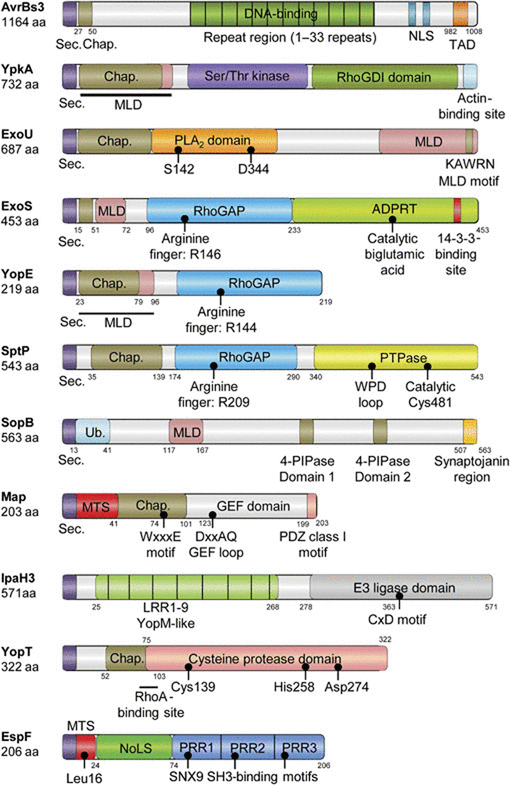
\includegraphics[width=0.6\textwidth]{img/architecture.jpg} 
\caption{Arquitectura de un conjunto de proteinas efectoras de bacterias. Algunos dominios identificables son: Sec. = secretion domain; Chap = chaperone-binding domain; PRR = proline-rich repeats. 
Se identifican otro tipo de módulos, por ejemplo motivos que pueden estar en cualquier parte de la secuencia. Figura extraída de \cite{dean2011functional}} 
\label{arquitectura}
\end{figure}









\subsection{Módulos proteicos} \label{modulosProteicos}
\subsubsection{Proteínas globulares}

% ESTRUCTURA
Las proteínas globulares son los compuestos proteicos más estudiados. En términos generales, estas proteínas se caracterizan por adoptar en condiciones nativas una conformación plegada compacta, 
dándole un aspecto globular y haciéndola soluble en el medio acuoso de la célula.

El hecho que sean, probablemente, las proteínas más estudiadas tiene que ver con todas estas propiedades estructurales básicas, 
al ser solubles y con una estructura determinada y relativamente estable, fueron las primeras que pudieron ser cristalizadas para luego resolver su estructura mediante difracción de rayos X.
La anotación de las estructuras que se resolvían permitió conocer mas sobre las propiedades estructurales mostrando que las proteínas globulares poseen una gran cantidad de estructuras secundarias interaccionando entre si, 
unidas por regiones de la secuencia con estructura flexible no determinada.

Las distintas estructuras secundarias se unen entre si mediante interacciones hidrofóbicas que involucran las cadenas laterales apolares, y por puentes de hidrógeno y a través de interacciones iónicas entre aminoácidos cargados, dando lugar
a la estructura compacta del plegamiento globular. Por lo tanto, el plegamiento adoptado por las estructuras secundarias(estructura terciaria) está intimamente asociado a las propiedades fisicoquímicas de la secuencia. 
En este plegamiento compacto, los aminoácidos más hidrofóbicos quedan alojados principalmente en el interior de la estructura, formando un núcleo hidrofóbico, 
y la superficie globular tiene mayoría de residuos polares, los cuales tienen la capacidad de interaccionar favorablemente con el solvente, lo que lo que le provee la solubilidad característica en el entorno celular. 

La estructura globular puede estar conformada por más de una cadena polipeptídica. En este caso, las diferentes subunidades se unen mediante las mismas interacciones que generan el plegamiento en una cadena, así, 
el plegamiento individual de una cadena puede contener aminoácidos con cadena lateral apolar en alguna región de su superficie, pero esta se complementa con la superficie hidrofóbica de otra cadena cuya interacción mantiene la estructura 
global del complejo.



% ASPECTOS ENERGÉTICOS, TERMODINAMICA Y PROCESO DE PLEGAMIENTO
Todas estas propiedades secuenciales diferenciales a lo largo de la estructura se asocian con el paradigma clásico de la biología estructural, el cual afirma que la secuencia primaria de una proteína 
contiene la codificación para que esta se pliegue adoptando una estructura tridimensional determinada y que, además, la conformación final se corresponde con un mínimo global sobre el perfil de energía libre asociado al polipéptido.  
Esta paradigma se deriva directamente al encontrar que al menos las proteínas pequeñas poseen una tendencia intrínseca a plegarse espontáneamente para dar una única estructura tridimensional.
Los detalles de este proceso de plegamiento, es decir, la forma en que el polipéptido sintetizado por el ribosoma recorre la superficie energética para alcanzar el estado plegado, ha inspirado una gran cantidad de estudios 
aunque aún hoy no se conoce en detalle el mecanismo subyacente.
% AGREGAR FIGURA DE SUPERFICIE ENERGÉTICA DEL PLEGAMIENTO

Teniendo en cuenta que adoptar una estructura determinada en un polipéptido implica un gran costo entrópico, y que las interacciones que describimos como estabilizadoras de este plegamiento son principalmente débiles, 
es de esperar que una característica de las proteínas globulares sea la capacidad intrínseca de su secuencia para formar gran cantidad de interacciones que permitan estabilizar la estructura plegada.





% PARADIGMA ESTRUCTURA FUNCION - PROPIEDADES DINÁMICAS DE LA ESTRUCTURA
El paradigma estructura-función original afirmaba que la función específica de una proteína está determinada por su estructura tridimensional, la cual es única y rígida. 
El origen de este paradigma es el modelo de llave-cerradura propuesto por Emil Fisher el 1894, 
que nace de la necesidad por por explicar la especificidad encontrada en el funcionamiento de diversas enzimas similares por sus correspondientes sustratos. 
La hipótesis utilizada para explicar esto era que la estructura de la proteína(en este caso la enzima) era perfectamente complementaria a la del sustrato correspondiente, en un sistema similar al de una llave en una cerradura.
% Este paradigma extiende los conocimientos vistos previamente acerca de que la secuencia de la proteína tiene codificada la información necesaria para plegarse espontáneamente luego de ser sintetizada en la célula,
% alcanzando esta estructura nativa asociada a la función.
Por un largo período de tiempo, entonces, el modelo de llave-cerradura y el paradigma asociado de estructura-función se mantuvieron como teorías aceptadas, confirmadas continuamente por la
gran diversidad de estructuras que se resolvieron mediante difracción con rayos X. 
% La capacidad de asociar una estructura única, encontrada en el cristal, con la función observada de la proteína en solución reforzaba la idea de una estructura estática asociada a las proteínas

Contrario a este modelo, en 1894 Koshlan sugiere el modelo de encaje inducido, basado en observaciones de enzimas que podían aceptar 
ligandos con diferentes estructuras y, por lo tanto, la proteína debía poseer cierta flexibilidad que le permitiera esta función.
Siguientes evidencias mostraron que esta flexibilidad era parte del mecanismo funcional y que podía implicar cambios conformacionales que van desde variaciones en rotámeros de las cadenas laterales hasta 
reordenamientos conformacionales muy relevantes(por ej. en proteínas alostéricas).
Estas variaciones podian aún ser interpretadas dentro del modelo establecido por el paradigma estructura-función, el cual fue levemente adaptado.
El requerimiento necesario para que la proteína cumpla su función era, entonces, una estructura definida, aunque dinámica. 
Por un tiempo todo pareció indicar(y la mayoría creyó) que una estructura definida, aunque dinámica, era la base del mecanismo funcional.

Si bien esta idea es una simplificación, dado que aún las proteínas mas estables son sistemas dinámicos con distintos grados de flexiblidad, este modelo se adapta a las funciones asociadas a proteínas globulares.
% Comenzaron a surgir, entonces, distintos modelos para explicar cómo la estructura tridimensional confería las propiedades necesarias para  
% Si bien esta idea es una simplificación, dado que aún las proteínas mas estables son sistemas dinámicos con distintos grados de flexiblidad, este modelo se adapta a una gran cantidad de proteínas.
En éstas, el ensamble conformado por los estados accesibles en condiciones fisiológicas está limitado a un conjunto de estructuras que solo difieren en leves desviaciones del promedio del ensamble.
La estructura resultante que se observa de la cristalización es, en realidad, un promedio del ensamble de conformaciones.

La dinámica de estas estructuras está dada por movimientos que van desde fluctuaciones rápidas de pequeña amplitud(del orden de \AA) hasta cambios relativamente lentos($\mu$s - $s$) que 
involucran modificaciones estructurales relevantes(plegamiento y movimientos asociados a la función).
Todos los movimientos son resultantes de rupturas y formaciones de interacciones provocadas por fuerzas de interacción las cuales, debido a su naturaleza débil, pueden romperse 
por efecto de la energía térmica, aún a temperatura ambiente. En general, todos estos movimientos están asociados al mecanismos por el cual ejercen su función.
% Por lo tanto, a pesar de que estas proteínas puedan ser asociadas con estructuras estáticas definidas, las más minimas fluctuaciones térmicas en condiciones normales les permiten
% explorar un conjunto relevante de conformaciones como parte de su actividad biológica.






% % CONCEPTOS EVOLUTIVOS DE LA ESTRUCTURA / SECUENCIA
Sabemos ahora que la funcionalidad emergente de los dominios globulares depende no solo de la estructura promedio del ensamble sino también de los aspectos dinámicos de ésta.
Todas estas características imponen requerimientos al mecanismo evolutivo ya que, para mantener la funcionalidad intrínseca de la proteína, se deben mantener los determinantes secuenciales y estructurales asociados al mecanismo funcional.
Esto impone ciertos requerimientos secuenciales y/o estructurales para la evolución de la proteína, que resulta en una similitud secuencial y estructural entre proteínas homólogas.

Estos conceptos han sido(y son) de gran ayuda en el estudio y clasificación de nuevas proteínas. 
Conociendo la estructura asociada a una proteína se puede inferir la funcion que desarrolla a partir de la búsqueda de proteínas con estructuras similares cuya función sea conocida.
Este mismo método se puede aplicar sobre dominios individuales ya que, como vimos, actúan como unidades estructurales y evolutivas individuales, mostrando funcionalidades independientes.

Incluso cuando no se conoce la estructura, los requerimientos estructurales imponen indirectamente restricciones sobre la secuencia (ya que la estructura es resultado directo de esta).
Estas, junto con ciertos determinantes secuenciales asociados directamente a la funcionalidad, forman un conjunto de restricciones impuesto sobre la evolución secuencial.
De esta forma, el mecanismo de comparación para inferir la funcionalidad puede ser utilizado de forma similar si se comparan las secuencia de una nueva proteína con la de otras cuya función es conocida.
Por lo tanto, la similitud secuencial también permite inferir propiedades funcionales, lo que facilita la anotación de elementos funcionales en secuencias nuevas, aún cuando no se conoce su estructura.

Dado que la secuencia está directamente ligada a la estructura resultante, la similitud secuencial entre proteínas es también un indicio de similitud estructural.
Estos conceptos asociados de propiedes secuenciales, estructurales y funcionales, unidos por el mecanismo evolutivo son las base de gran parte del conocimiento actual sobre proteínas globulares.

% Más alla de esto, los análisis de estructuras existentes asociadas a proteínas globulares permitieron encontrar que hay una gran conservación en los diseños de arquitectura.
% Las combinaciones de estructuras secundarias que daban lugar al plegamiento podían agruparse, entonces, en conjuntos de arquitecturas globales de la proteína que permite
% clasificar y anotar las proteínas de acuerdo a estas arquitecturas resultantes.
% Como resultado de estos analisis estructurales se desarrollaron diversas clasificaciones y bases de datos asociadas. 
% Ejemplo de estas son SCOP y CATH, las cuales se basan en la topología emergente de la combinación de estructuras secundarias propia de la proteína para armar clasificaciones jerárquicas de la arquitectura.
% En el nivel más bajo de la clasificación se encuentran estructuras con gran similitud entre si, indicativo de un ancestro en común y agrupadas generalmente por funciones idénticas o similares.
% % Esta agrupación en ``familias'' con alta  es posible porque, aún cuando la secuencia pueda sufrir mutaciones, la estructura debe conservarse para mantener la funcionalidad.
% 
% % Incluso cuando ....The sequences diverge, but the overall domain architecture remains the same.
% % Particular domains and domain architectures are well conserved over the course of evolution. 






% ACTIVIDADES
Como se menciono previamente el perfil de actividades biológicas asociadas a las proteínas globulares está directamente relacionado con las propiedades conformacionales de estas.
En general, las funciones más estudiadas están asociadas con actividades enzimáticas, donde las proteínas se encuentran generalmente solubles en el medio acuoso de la célula.
La estructura tridimensional definida y gran tamaño que pueden alcanzar estas proteínas también les permite intervenir en actividades que requieren interacciones específicas y estables con otras moléculas, 
ejemplo de esto son los anticuerpos y las proteínas que intervienen en la replicación y reparación del ADN.
El gran tamaño y la solubilidad le permiten actuar como transportadores de otras moléculas con baja solubilidad en medio acuoso.

Las flexibilidad estructural permite que se experimenten cambios conformacionales considerables en la estructura terciaria. 
Dado que las propiedades conformacionales están intimamente ligadas a la funcionalidad, estos cambios, 
que pueden ocurrir como producto de la unión de ligandos o modificaciones sobre químicas dinámicas sin alterar la secuencia, permiten ejercer efectos regulatorios sobre la actividad de la proteína.






% 
% – Flexibilidad
% • No son estructuras rígidas
% • Su flexibilidad depende de un gran número de enlaces débiles
% 
% – Interacciones
% • Unión reversible de ligandos
% • Interacciones reversibles proteína-proteína
% • Se llevan a cabo mediante enlaces débile
% 















\subsubsection{Proteínas de membrana}
Las proteínas de membrana se definen como cualquier proteína que interacciona con la membrana lipídica de la célula.
Algunas de estas proteínas están unidas solo a la superficie de la membrana, mientras que otras tienen regiones que se insertan en el núcleo hidrofóbico(y, posiblemente, también contiene dominios por fuera de éste). 
Se puede hacer, entonces, una primera clasificación en 2 grupos: proteinas integrales y periféricas.

Las proteínas extrínsecas(o periféricas) no interaccionan con el núcleo hidrofóbico y tienen propiedades estructurales y secuenciales similares a las proteínas globulares, 
pero se mantienen en constante interacción con la membrana mediante distintos mecanismos.
Algunas interaccionan indirectamente mediante la unión a proteinas integrales de membrana, otras lo hacen a través de la interacción con los grupos polares que componen las cabezas de los fosfolípidos en la membrana. 
Otro conjunto de proteína periféricas atraviesan procesos de modificaciones post-traduccionales que las unen covalentemente a cadenas carbonadas, las cuales pueden insertarse en el núcleo hidrofóbico y
asi mantener a la proteína en constante interacción con la membrana.
En general, esta clase de proteínas tiene actividades biológicas asociadas a la unión a la membrana, por ejemplo transducción de señales extracelulares, están involucradas en la cadena de transporte de electrones, etc.

% ESTRUCTURA
El otro conjunto de proteínas de membrana son las proteínas integrales(o intrínsecas) tienen uno o mas segmentos insertos en la bicapa lipídica.
En la mayoria, la región insertada atraviesa la membrana (proteínas transmembrana) y tienen dominios intra y extra celulares.
A partir de estos conceptos generales se puede deducir que esta clase de proteínas tendrá una arquitectura/topología particular, donde 

Los segmentos que atraviesan permiten hacer una nueva clasificación por si mismos, así, las proteínas transmembrana se pueden agrupar en dos conjuntos según la estructura que les permite atravesar el núcleo hidrofóbico.
Un primer conjunto de proteínas, las porinas, contienen una estructura característica compuesta por hebras-$\beta$ en una conformación característica con forma de barril que atraviesa la membrana, formando una expansión similar a un poro.
Los aminoácidos de la secuencia son generalmente polares pero, a diferencia de las proteínas globulares típicas, los grupos laterales que están en contacto con la cara externa del barril son hidrofóbicos, y son los que están en contacto con 
los grupos lipídicos, mientras que las cadenas laterales hidrofílicas se encuentran mirando hacia el interior del poro.
La actividad biológica de estas proteínas se deriva directamente de esta estructura, las porinas forman canales en la membrana a través de los cuales distintos metabolitos solubles en agua pueden atravesarla. 

El otro conjunto está dado por aquellas proteínas que contienen hélices-$\alpha$ atravesando una o mas veces la membrana. 
Esta estructura secundaria es la más común entre los segmentos transmembrana ya que permite permite satisfacer todos los puentes de hidrógeno caracterísicos de la estructura carbonada de
the helical structure can satisfy all backbone hydrogen-bonds internally, 
sin dejar grupos polares expuestos hacia fuera de la hélice, y por lo tanto, en contacto con el núcleo hidrofóbico de la membrana

Estos dominios transmembrana tienen, por lo tanto, propiedades secuenciales particulares caracterizadas por aminoácidos con cadenas laterales hidrofóbicas que les permiten interaccionar con el núcleo de la membrana.
% y, generalmente, también con los grupos polares en las superficies de ésta.
Un ejemplo común de este tipo de proteínas es la glicoforina, que contiene un segmento con estructura de hélice-$\alpha$ compuesto totalmente de residuos hidrifóbicos. 
Esta hélice hidrofóbica está, además, rodeada por segmentos flanqueantes conteniendo aminoácidos cargados que interaccionan con las cabezas polares de los fosfolípidos y previenen que la proteína se deslice,
manteniéndola inserta en la membrana.
% Las propiedades hidrofóbicas de su superficie, la flexibilidad que poseen en sus estructuras de forma aislada(no insertadas en la membrana) y los bajos niveles de expresión hacen que sean difíciles de cristalizar.
% Por lo tanto, el estudio de sus estructuras siempre estuvo retrasado con respecto al de las proteínas globulares.
Dentro de este último conjunto existe una gran cantidad de proteínas que contienen múltiples hélices-$\alpha$ transmembrana. Estás proteínas generalmente están conformadas de 2 hélices(formando una estructura tipo coiled-coil)
o 7 hélices(en un arreglo característico de proteínas como la rodopsina).

Estas particularidades en la secuencia permiten distinguirlas fácilmente de, por ejemplo, las proteínas globulares. 
Además, a partir de estos módulos transmembrana y extra/intra celulares se pueden clasificar estas proteínas según la arquitectura o topología global, de acuerdo al número y tipo de segmentos transmembrana, etc.



















\subsubsection{Proteínas intrínsecamente desordenadas}


%  CONCEPTOS GENERALES, SIMPLEMENTE PARA INDICAR QUE NO TIENEN UNA ESTRUCTURA TRIDIMENSIONAL DEFINIDA
% ******************************
Los conocimientos acerca del proceso de plegamiento y la estructura resultante derivados de proteinas globulares formaron, durante un largo tiempo, ideas que se creían aplicables a todas las proteínas existentes.
Con el tiempo se encontraron proteínas que, al parecer, ejercían su función sin tener una estructura tridimensional determinada. 
Estas ideas no se adaptaban a las características de plegamiento y al paradigma estructura-función reinante, por lo tanto, fueron identificándose 
y estudiándose experimentalmente una a una, tratándolas como excepciones al modelo clásico.
Luego de este proceso, hace al menos una década, se formalizó la idea que el estado adoptado en condiciones nativas(funcionales) de muchas regiones o proteínas enteras podía ser intrínsecamente desordenado
(IDRs/IDPs = intrinsically disordered regions/proteins, a partir de ahora). 
% Es decir, existe un conjunto cada vez mas amplio de proteinas cuya secuencia no codifica un plegamiento determinado.



% Inicialmente, gran cantidad de evidencia soportaba la idea que la funcionalidad de las proteínas estaba asociada a su estructura tridimensional bien definida pero dinámica.
% Al no tener una estructura tridimensional determinada, el paradigma reinante que implicaba la necesidad de ésta para poder cumplir alguna función biológica no permitía incluirlas como parte del proteoma.
% Consecuentemente, la idea de que muchas proteínas o regiones no adopten una estructura definida y posean una conformación intrínsecamente desordenada se creyó inaceptable. 
% Estamos hablando de un numero considerable de proteinas cuya secuencia encodes for the intrinsically unstructured proteins without specific structure.
Este reconocimiento trajo consigo una gran cantidad de preguntas, relacionadas con las características estructurales de éstas:
¿Que tan desordenadas/desplegadas son estas proteínas?, ¿Son realmente conformaciones aleatorias o conservan una estructura residual?
¿Si poseen una estructura residual, cómo se clasifican sus conformaciones?
Los avances sobre estas preguntas iban mas allá de las técnicas de resolución estructural conocidas que estaban basadas en el promedio del ensamble, quedando, entonces,
a la espera de aproximaciones/conocimientos provenientes de nuevas técnicas del campo de la biofísica\cite{eliezer2009biophysical}.




% ******************************
% PROPIEDADES ESTRUCTURALES
% ******************************

% CONCEPTOS GENERALES !!! REESCRIBIR-REORDENAR

Este conjunto de proteínas desordenadas se caracteriza la tendencia a adoptar conformaciones extendidas con bajo contenido de estructura secundarias.
La principal característica distintiva de las IDPs es, entonces, su inhabilidad para plegarse en una estructura tridimensional única.
En algunos casos, sin embargo, pueden formar estructuras desordenadas pero compactas, y algunos segmentos de la secuencia pueden adoptar transitivamente estructuras secundarias individuales.
Como vamos a ver, esta leve estructura residual(latente o transitiva) es muy importante y representa gran parte de las capacidades funcionales en IDRs/IDPs.
A pesar de esta tendencia desordenada, debido a la naturaleza heteropolimérica de las proteínas, es probable que las IDPS adopten conformaciones totalmente aleatorias(donde las conformaciones solo estan restringidas por impedimentos estéricos),
aún en entornos altamente desnaturalizantes donde normalmente se pierden las propiedades estructurales.
Por lo tanto, se puede ver que las IDPs poseen propiedades conformacionales complejas, y que esta 
excepcional heterogeneidad estructural representa tambien un problema crítico a la hora de estudiarlas experimentalmente y caracterizarlas.
% Por lo tanto, se puede decir que las IDPs poseen propiedades conformacionales mucho mas complejos que polipéptidos con estructuras totalmente aleatorias y que esta 




% Thus, coil-like ID proteins are not completely random, but are characterized by the presence of some residual (and highly flexible) structure. 

% A partir de esta descripcion estructural se puede entender por qué el término inicial asignado a estas proteínas (proteínas desestructuradas) ha quedado obsoleto.

% A pesar de esta falta de estructura única definida, como se vió, presentan una gran diversidad de propiedades estructurales y, lo que es mas importante, estas están relacionadas con las funciones de la proteína. 
% Por lo tanto, el término general para describir estas proteínas es, simplemente, ``desordenadas''. 
% Este término se aplica tanto a las regiones que forman parte de proteinas plegadas mas grandes, como a secuencias que carecen totalmente de estructura plegada. 
% Como veremos, el mosaico estructural que ofrece la variedad de secuencias conformadas por regiones con propiedades estructurales diversas es fundamental para obtener el extenso catálogo de funcionalidades existentes.    



% Ahora que sabemos que las IDRs/IDPs no están completamente libres de restricciones estructurales, nos concentraremos en describir cuales son las características de su conformación:
Una característica resultante de estas propiedades es que las IDPs poseen conformaciones altamente dinámicas con estructuras que se interconvierten en diferentes escalas de tiempo. 
Estas estructuras varían desde estados completamente sin estructura(polipéptidos nativos sin plegamiento) hasta estados parcialmente plegados(sin estructuras secundarias definidas), o incluso ensambles desordenados pero con ciertas
estructuras secundarias claramente determinadas.
La distribución de estas estructuras está cambiando continuamente en el tiempo, es decir, la estructura tridimensional que podemos ver en un instante dado será diferente de la que veremos en otro momento.

% A pesar de esta dinámica estructural, sin embargo, las IDRs/IDPs carecen de cualquier tipo de estructura secundiaria(o terciaria) estable bajo condiciones fisiológicas.
% Las estructuras residuales que describimos como parte del ensamble, a pesar de ser transitorias, tienen un papel relevante en el cumplimiento de la función asociada a la proteína.
% Cualquier IDR/IDP contiene una gran cantidad de este tipo de elementos estructurales, algunos con gran potencial para plegarse, otros con capacidades de plegamiento diferencial(en algún contexto determinado) 
% y otros sin posibilidad alguna de adquirir una estructura determinada.
% De esta última descripción se puede imaginar que, probablemente, ningún IDR/IDP adoptará una conformación totalmente desordenada a lo largo del tiempo(aunque tampoco estará completamente plegada), por el contrario, se tendrá una gran variedad
% de posibles mosaicos con distintas proporciones y tipos de elementos estructurales.


Estas propiedades dinámicas se pueden entender fácilmente a partir del perfil energético característicamente asociado a estas proteínas.
% En la parte derecha de la figura \ref{idpBindingEnLandscape} se representa gráficamente el perfil energético asociado a estas propiedades conformacionales.
Como se puede ver en la figura \ref{idpBindingEnLandscape}, el paisaje entero queda descrito por una superficie semiplana con múltiples conformaciones asociadas al mínimo de energía, 
con valores de energía aproximadamente iguales y separados por barreras energéticas muy pequeñas.
Estas barreras representan las transiciones rápidas y frecuentes entre las distintas conformaciones que resultan en las propiedades observadas experimentalmente
en solución: un conjunto heterogéneo de conformaciones fácilmente maleable por cambios en el medio. 
En base a esto, se ve que una descripción detallada de IDPs requeriría conocer el ensamble de estados posibles junto con las velocidades de interconversión entre estos.
Todas estas propiedades y las velocidades de las transiciones en el ensamble son difíciles de capturar experimentalmente(y computacionalmente también), aún usando técnicas experimentales que no se basan en promedios de conformaciones.
Los estudios sobre este tipo de proteínas, entonces, se han enfocado en analizar los estados termodinámicamente accesibles como entidades discretas.
Esta idea, si bien sabemos que es una descripción incompleta, permite modelar de forma discreta los elementos funcionales relevantes, sirviendo como base para estudios posteriores.
Este modelo puede extenderse si se representan también las probabilidades de ocurrencia para distintas conformaciones individuales en el ensamble, obteniendo asi un modelo mas dinámico del sistema.



% ***************
%  INDUCED FIT:
% ****************
% Además, este perfil energético se ve modificado por distintas condiciones como modificaciones post-traduccionales, condiciones del medio, presencia de ligandos,etc.
Además, estos ensambles conformacionales dinámicos pueden verse modificados por distintas situaciones como cambios en las condiciones del entorno, modificaciones post-traduccionales, presencia de ligandos, etc.,
lo que modifica no sólo los estados accesibles, sino también la distribución de poblaciones que se encuentran en cada uno.
Una propiedad particular dependiente del contexto, encontrada en los ensambles conformacionales asociados a IDPs, es la capacidad de adquirir nuevos elementos estructurales ordenados estables luego de la unión a ciertos ligandos
(proceso conocido como textit{binding \& folding}\cite{dyson2005intrinsically}). 
Esta propiedad se hace mas relevante de investigar cuando se sabe que, generalmente, está asociada a su funcionalidad biológica y ocurre previamente o durante la realización de esta función.
% Although disordered proteins exist as dynamic structural ensembles without fixed(estable!!!) tertiary structures, there is evidence that many flexible regions of proteins undergo coupled binding and folding \cite{dyson2005intrinsically}. 
% A large decrease in conformation entropy accompanies such disorder-to-order transitions. 

Una gran cantidad de IDPs, entonces, se ven estabilizadas termodinámicamente mediante la unión a ligandos específicos(generalmente otras proteínas, DNA, membranas, etc)
% In other words, intrinsically unfolded proteins in vivo are likely to be stabilized by functional binding to specific targets and ligands 
% (such as a variety of small molecules, substrates, cofactors, other proteins, nucleic acids, membranes and so on). 
% Many intrinsically disordered proteins undergo transitions to more ordered states or fold into stable secondary or tertiary structures on binding to their targets — that is, they undergo coupled folding and binding processes.
Los complejos funcionales entre IDPs y sus ligandos son formados por interacciones intermoleculares específicas y modifican el paisaje energético visto previamente, generando nuevos estados definidos de mínima energía.
Esta diferencia se ve en la región izquierda de la figura \ref{idpBindingEnLandscape}.


\begin{figure}[h]
\centering
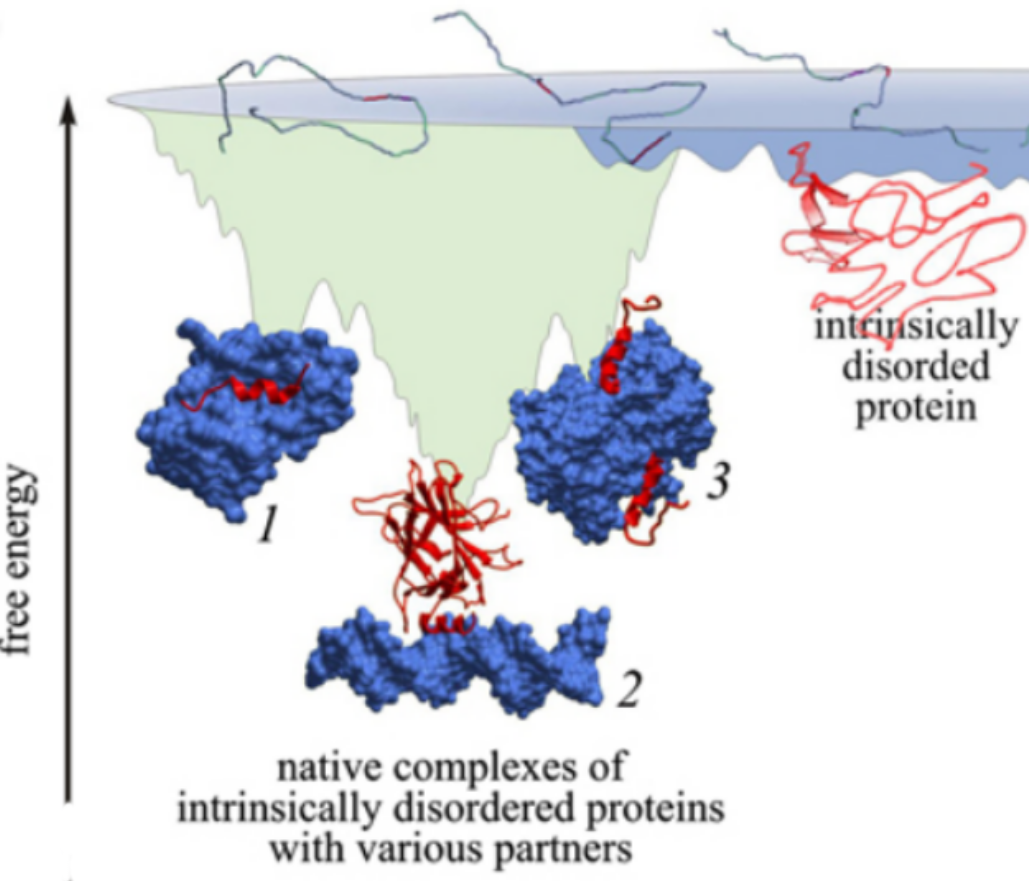
\includegraphics[width=0.7\textwidth]{img/idp-binding-EnLandscape2.png} 
\caption{Perfil energético de los estados de IDRs/IDPs. Los segmentos desordenados pueden plegarse para dar estructuras ordenadas estables a través de interacciones con ligandos específicos.
Esta situación se da cuando la formación del complejo resulta en una disminución de energía libre. 
% Disordered segments of these proteins can gain ordered structure at the interaction with specific binding partners in a case if the free energy of such complexes is lower 
% than the free energies of the intrinsically disordered protein and its partner. 
Por si sólo, el polipéptido presenta un paisaje energético semiplano(sección derecha). La interacción con distintos ligandos(1,2,3) resulta en nuevos estados termodinámicamente estables.
Figura extraída de \cite{turoverov2010protein}}
\label{idpBindingEnLandscape}
\end{figure}

Las IDPs pueden adoptar esta conformación plegada si la energia del complejo formado es menor que la energía libre correspondiente al segmento desordenado y su ligando, previo a la interacción.
% IDPs fold as a whole while interacting with their partners, if the free energy of complex is lower than the free energies of IDP and its partner before their interaction.
En general, sólo un segmento desordenado con características anfipáticas es el que está involucrado en el proceso de unión y plegamiento, en este caso el segmento se denomina elemento de reconocimiento(RE=recognition element). 
% More often, however, only a part of an IDP, a specific recognition element, which is a relatively short amphipathic linear motif contained within long disordered sequence, is involved in the coupled folding and binding events
% Induced fit interactions can also occur between structural domains and relatively large natively unstructured regions of other proteins. 
% The natively unstructured region is then induced to form a stable structure, but only in the presence of the interacting structural domain.
Este tipo de transiciones ante la unión a ciertos ligandos, involucrando regiones cortas de la secuencia, provee una combinación de alta especificidad y baja afinidad que hace a este tipo de elementos extremadamente útiles en procesos de señalizacion y regulación.
% This disorder-to-order transitions, in turn, leads to a combination of high specificity and weak affinity, a pair of linked features that are extremely useful for signalling and regulation.

Una pregunta que aparece naturalmente al intentar estudiar este proceso es si el elemento estructural ordenado es generado durante la unión al ligando 
o si pertenece al conjunto de elementos estructurales encontrados transitivamente en las IDRs/IDPs y, al unirse, se hace parte de la conformación estable.
% An often-raised issue with respect to IDP binding is whether folding occurs before or after binding (termed conformational selection and induced folding, respectively).
% Detailed studies suggest that folding can occur both before and after binding in distinct cases
Estas dos opciones se reflejan en los modelos de selección de conformación y el de unión y plegamiento simultáneo.
Obviamente, en la realidad puede ocurrir cualquiera de estos dos mecanismos o una combinación de los dos.
Esto se ve representado en la figura \ref{idpBinding}


\begin{figure}[h]
\centering
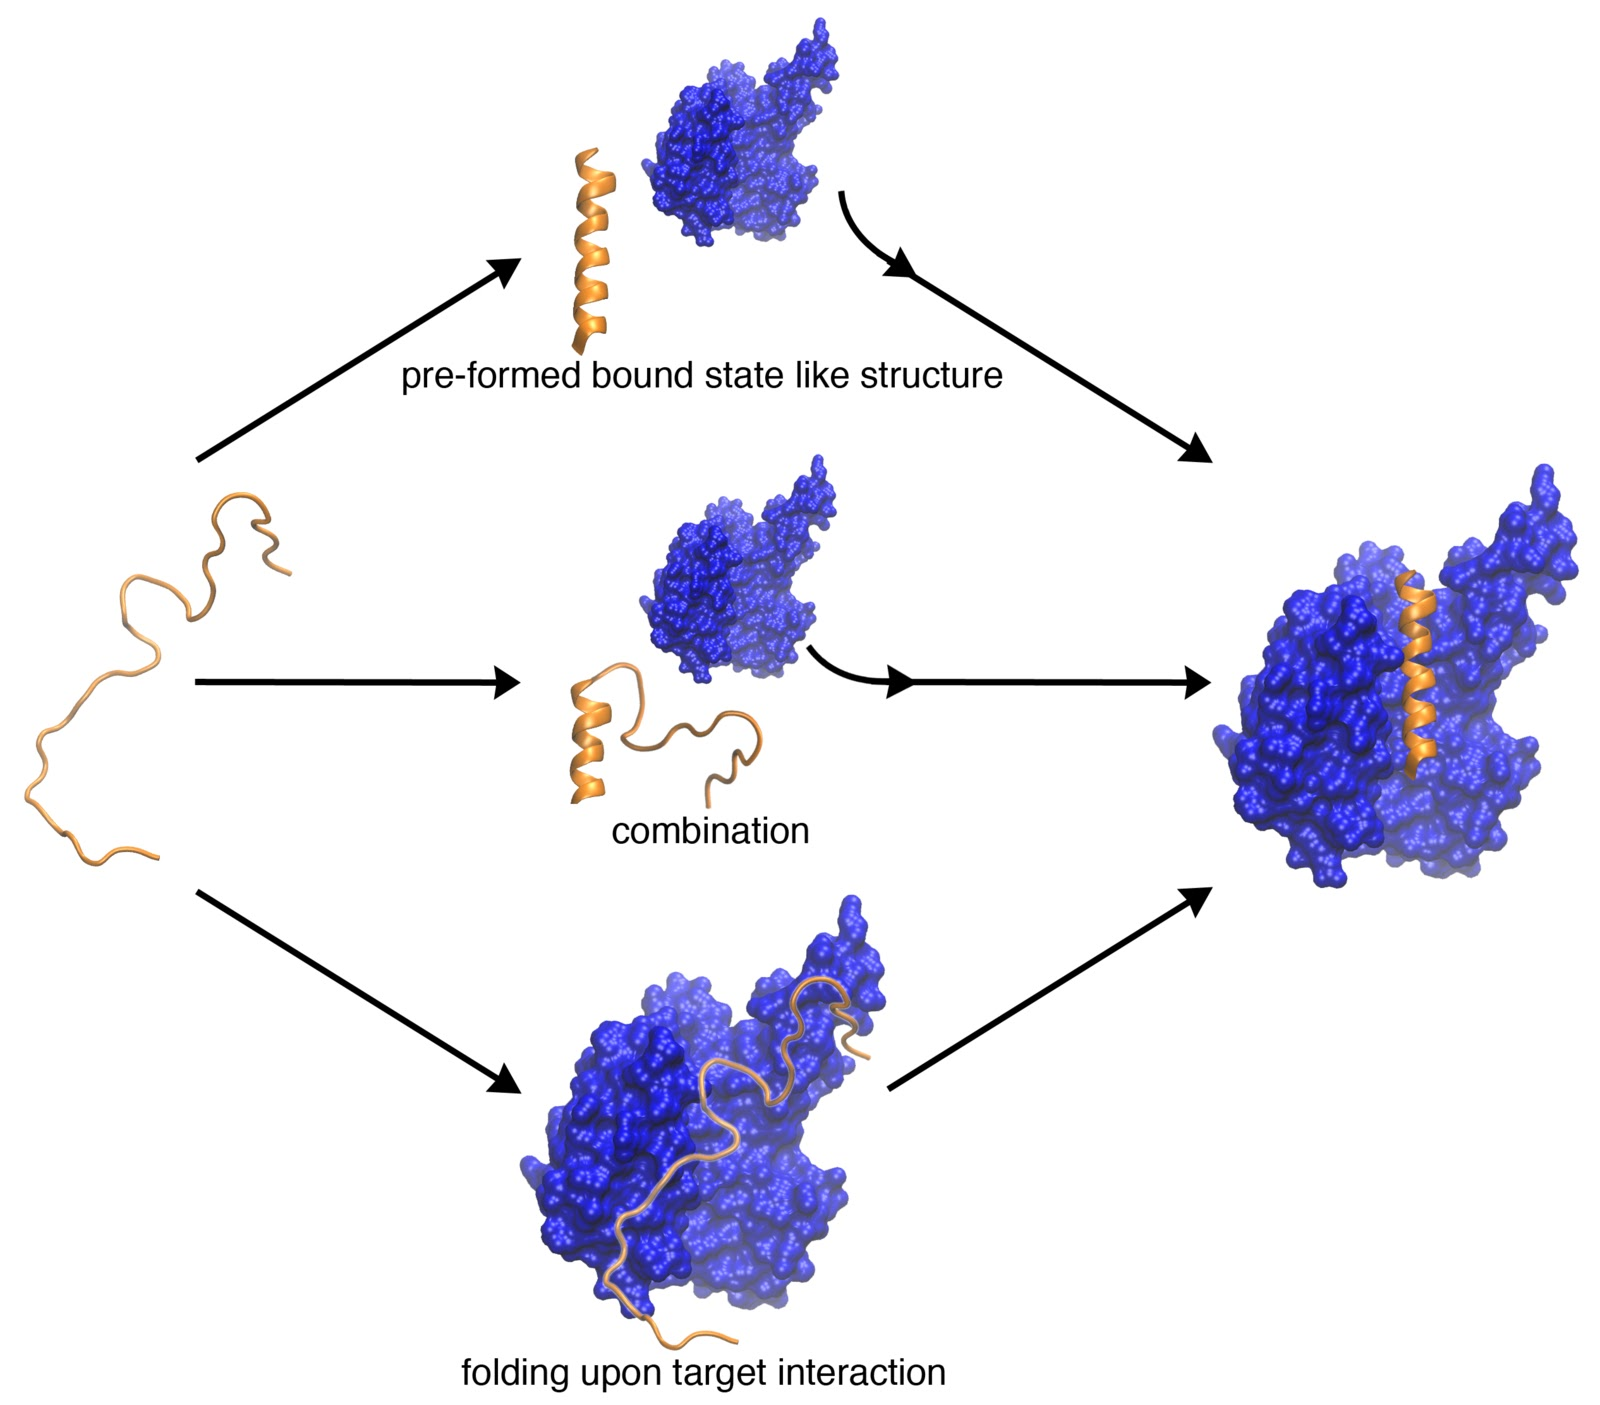
\includegraphics[width=0.8\textwidth]{img/PSE-MoRE.jpg} 
\caption{Distintos modelos de \textit{binding \& folding}} 
\label{idpBinding}
\end{figure}



% ESTO TIENE QUE IR DESPUES DE TODO EL DESARROLLO DE INDUCED FIT
% En base a estas propiedades estructurales y el induced fit, en el review \cite{dunker2001intrinsically} se plantea una clasificacion del desorden en dos categorias: intermittent and constant.
% The former describes protein molecular recognition domains and other regions that undergo order/disorder transitions to carry out binding or other functions. The latter describes regions such as
% proteinaceous detergents, flexible linkers, entropic springs, entropic clocks and entropic bristles that remain disordered while carrying out function.

A partir del estudio sobre este proceso de 'binding \& folding', basándose en los modelos previos, se encontraron algunos conceptos importantes inesperados.
En primer lugar se encontró que dos IDRs/IDPs pueden unirse en un proceso de unión y plegado mutuo \cite{bhattacherjee2012coupled},
es decir, una IDR/IDP también puede funcionar como ligando y plegarse en este proceso. 
Por otro lado, se encontró que el proceso de unión y reconocimiento del ligando puede proceder aún sin necesidad de plegamiento. 
Esto tiene implicancias importantes en los aspectos funcionales ya que, como se había predicho, la capacidad de unión a ligandos dependía de la formación de este elemento estructural.
Gran cantidad de ejemplos de este tipo de uniones(determinados complejos ``fuzzy'') extienden la idea de desorden no sólo a proteínas en solución, sino también a interacciones formando complejos. 









% PROPIEDADES SECUENCIALES
Muchos estudios se hicieron para intentar identificar cómo las características  estructurales tan particulares de las IDPs están codificadas en la secuencia de la proteína.
En el caso de las proteína globulares, la secuencia primaria codifica el proceso de plegamiento y, a través de este, la estructura única final. 
De forma similar, al identificar la IDPs cómo entidades estructuralmente diferenciables, se podría pensar que la estructura primaria de estas determina, también, su falta de estructura tridimensional definida.
Esto tiene como corolario la idea que las secuencias de ambos conjuntos (proteinas ordenadas y proteínas desordenadas) deberían ser diferenciables entre si.
La ausencia de una estructura definida en IDPs es atribuida a las características particulares de sus secuencias de aminoácidos las cuales se describen como secuencias de baja complejidad, enriquecidas en aminoácidos 
cargados y polares, junto con Glicina y Prolina, y un bajo contenido de residuos hidrofóbicos. 
La secuencia suele tener una alta carga neta(positiva o negativa) resultante, o tener segmentos separados de residuos cada uno cargas positivas o negativas.
% Durante el proceso de descubrimiento del conjunto IDPs, muchas proteínas fueron identificadas inicialmente debido a estas simples diferencias en la secuencia.
La relación entre esta combinación de baja hidrofobicidad y alta carga neta y la falta de una estructura definida puede explicarse desde el punto de vista físico:
los altos valores de carga neta producen efectos de repulsión entre las cargas de los residuos, mientras que la baja hidrofobicidad previene la compactación de la estructura lineal
(las interacciones hidrofóbicas son una de las principales fuerzas que interviene en el proceso de plegamiento).
De esta forma, las IDPs no poseen las propiedades secuenciales que le permitan formar suficientes interacciones para estabilizar una estructura compacta con un núcleo hidrofóbico, característica de las proteínas globulares.
% Estas propiedades no solo son necesarias para estabilizar la estructura compacta final sino que también se cree son importantes en el proceso de plegamiento para adquirir esta estructura.
% en un proceso similar a un colapso hidrofóbico. 
El resultado es una estructura con tendencia a mantener una conformación desplegada, característica de las IDPs.

 
% ****SI HACE FALTA PUEDO AGREGAR ESTE PARRAFO SOBRE ALGUNAS CARACTERISTICAS EXTRA DE LAS SECUENCIAS, O REFERENCIAR ALGO, 
% 
% The disordered proteins are significantly depleted in bulky hydrophobic (Ile, Leu, and Val) and aromatic amino acid residues (Trp, Tyr, and Phe), which would normally form the hydrophobic core of a folded globular protein, 
% and also possess low content of Cys and Asn residues.
% The depletion of ID protein in Cys is also crucial as this amino acid residue is known to have a significant contribution to the protein conformation stability via 
% the disulfide bond formation or being involved in coordination of different prosthetic groups.
% On the other hand, ID proteins were shown to be substantially enriched in polar, disorder-promoting, 
% amino acids: Ala, Arg, Gly, Gln, Ser, Glu, and Lys and also in the hydrophobic, but structure braking Pro.


% The fact that natively unfolded proteins, with their depleted hydrophobicity, are noncompact under physiological conditions indicates that ‘salted water’ (typical ‘physiological’ buffer contains 100–150 mM NaCl) does not represent for them a poor solvent.
% In other words, these conditions do not force polymer segments to interact specifically with each other and, thus, do not force them to be effectively excluded from the solvent.
% On the other hand, it has already been noted that even high concentrations of strong denaturants do not represent a good solvent for a polypeptide chain encoding for a typical globular protein, and a globular protein was assumed to never be a random coil.


% Por lo tanto, a signature of probable intrinsic disorder is the presence of low sequence complexity and amino-acid compositional bias, with a low content of bulky hydrophobic aminoacids (Val, Leu, Ile, Met, Phe, Trp and Tyr), which would
% normally form the core of a folded globular protein, and a high proportion of particular polar and charged amino.....
% ESTAS PROPIEDADES SE HAN UTILIZADO PARA LAS PRIMERAS GENERACIONES DE HERRAMIENTAS PARA PREDECIR DESORDEN A PARTIR DE LA SECUENCIA.
% Luego se crearon predictores que analizaban la secuencia usando ventanas(PONDR)

% In addition to amino-acid composition, the disordered segments have also been compared with the ordered ones by various attributes such as hydropathy, net charge, flexibility index, helix
% propensities, strand propensities, and compositions for groups of amino acids such as W + Y + F (aromaticity).

% Estas propiedades fisicoquimicas tambien fueron incluidas para los predictores.













% ACTIVIDADES
% 
% % Como vimos antes, diversos estudios estructurales mostraron que este tipo de conformaciones no solamente existe realmente \textit{in-vivo}, sino que representa el estado funcional de estas proteínas y,
% % dado que la habilidad para realizar su función biológica es lo que distingue al estado nativo, este conjunto de proteínas parcial o totalmente desordenadas debe ser considerada como entidades nativas. 
% Debido a su amplio ensamble conformacional, el cual va más allá de una simple variación/dinámica estructural, el modelo de encaje inducido al cual se adaptan correctamente las proteínas globulares no permitiría explicar el funcionamiento
% de las proteínas intrínsecamente desordenadas.
% Por lo tanto, estas proteínas desafían el paradigma casi dogmático de estructura-función, fuertemente establecido hasta el momento.
% Esto significa que el paradigma estructura-función previo, que implica la indispensable existencia de una estructura ordenada como requisito para una función efectiva, debe ser redefinido para incluir ese nuevo conjunto de entidades
% \cite{wright1999intrinsically}.
% De acuerdo a este nuevo paradigma, las proteínas nativas(o sus regiones funcionales) pueden existir en cualquiera de los estados conformacionales conocidos que se desarrollaron en las secciones previas.
% En la figura \ref{stuctured-idp-functions} se muestra el paralelismo entre los paradigmas descritos y el proteoma resultante.
% 
% 
% \begin{figure}[h!,centered]
% \centering
% 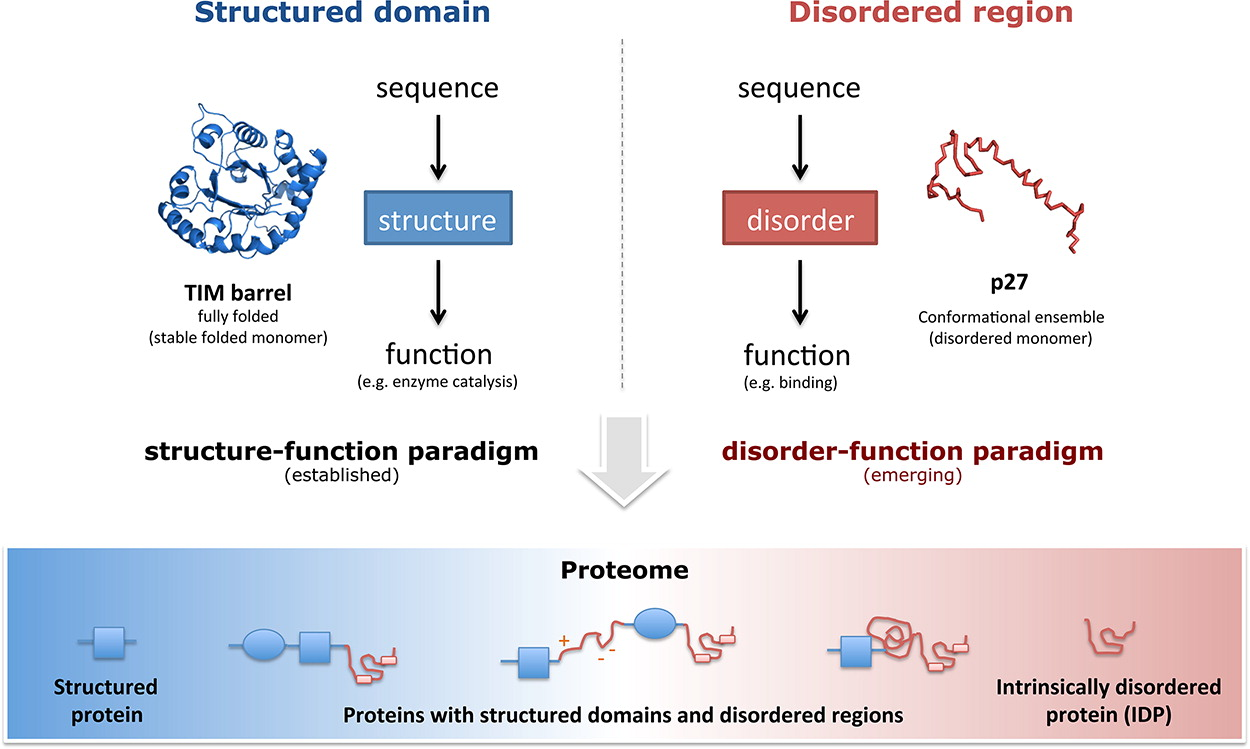
\includegraphics[width=0.9\textwidth]{img/structure-idp-function.jpeg} 
% \caption{Paralelismo entre funcionalidad emergente de dominios plegados y de proteinas/regiones intrínsecamente desordenadas. Figura extraida de \cite{van2014classification}}
% \label{stuctured-idp-functions}
% \end{figure}


% El principal objetivo de todos los modelos y estudios estructurales en estas proteínas es poder elucidar los tipos y modos funcionales subyacentes.
Una pregunta importante que surge de las propiedades estructurales es como estas desarrollan las funcionalidades asociadas y cuales son las funciones fisiológica que cumplen las IDPs.
% El estudio de las funcionalidades provistas por IDPs se ve dificultada por las propiedades intrínsecas de estas proteinas:
% Como se dijo antes, el paradigma inicial de secuencia-estructura-función provee una base para relacionar los conocimientos entre mediante métodos de análisis y anotaciones de secuencias estructuras y funciones.
% Por el contrario, las proteínas dentro de este nuevo conjunto de IDPs se corresponden con un ensamble conformacional heterogéneo.
% Dado que, entonces, no es posible obtener una estructura promedio representativa, es díficil obtener información relevante de la funcionalidad a partir del ensamble conformacional.
% Lo que es más, dada la ausencia de restricciones estructurales, las secuencias de estas proteínas tienden a evolucionar más rapidamente que sus pares ordenados.
% Como resultado, la identificacion de secuencias/regiones homólogas es considerablemente mas difícil.
% Estas consideraciones manifiestan la necesidad de avanzar en el desarrollo de esquemas de clasificación específicos para este nuevo conjunto de proteínas, apuntando a mejorar la predicción funcional y la anotación.
Un paso importante para entender esto es la clasificación de las IDPs conocidas de acuerdo a sus funcionalidades\cite{van2014classification}.
% Como parte de estos avances se han ensayado una gran diversidad de clasificaciones\cite{van2014classification}.
La figura \ref{idpFunctions} detalla la clasificacion de funcionalidades y mecanismos asociados a IDPs junto con las proporciones de instancias encontradas para cada uno.
De esta clasificacion se puede ver que las funcionalidades en las IDPs emergen a partir del propio desorden intrínseco o mediante mecanismos de reconocimiento molecular(interacciones transitivas o permanentes).
% En la figura \ref{proteinMechanisms} se ve una clasificación general bastante simplificada de los roles y mecanismos funcionales generalmente provistos por los distintos tipos de proteinas. 
% En esta clasificacion de proteinas segun su rol general, se incluyen también las proteínas globulares y de membrana que mencionamos previamente(asociadas a actividades enzimáticas, transporte, etc), agrupadas como proteínas plegadas.

En el primero caso, el mecanismo subyacente de funcionamiento no implica ninguna interacción sino que depende directamente de la flexibilidad y plasticidad de la cadena carbonada(\textit{entropic chains}).
En este caso, las proteínas satisfacen un conjunto de requerimientos celulares únicos en los cuales la funcion a cumplir es una consecuencia directa de las propiedades conformacionales que poseen. 
Esta función, generalmente está asociada a secuencias linkers, cuyo objetivo es unir distintos unidades componentes de las proteínas.

En el segundo caso, el amplio perfil de interacciones posibles permite que las IDPs participen en funcionalidades muy diversas, entre estas están la función de chaperonas, la modulación de actividades de otras moléculas(generalmente proteínas) 
y la neutralización de pequeños ligandos uniéndose a ellos.
% El mecanismo asociado a estos generalmente implica el plegamiento para adquirir una estructura ordenada al interaccionar con el ligando.
El mecanismo de reconocimiento e interacción es básicamente diferente a la que adoptan los dominios globulares. 
Mientras que estos últimos han evolucionado para dar una gran variedad de plegamientos diferentes que proveen reconocimientos especificos, 
en IDPs el mecanismo de unión \textit{binding} es principalmente mediado por segmentos cortos de reconocimiento\cite{neduva2005systematic,fuxreiter2007local}, caracterizados por su naturaleza flexible, lo que 
les aporta una gran cantidad de ventajas\cite{gunasekaran2003extended,dyson2005intrinsically}.%REFERENCIA AL PAPER DE MECANISMOS FUNCIOMNALES DE IDPs

% 
% \begin{figure}[h!,centered]
% \centering
% 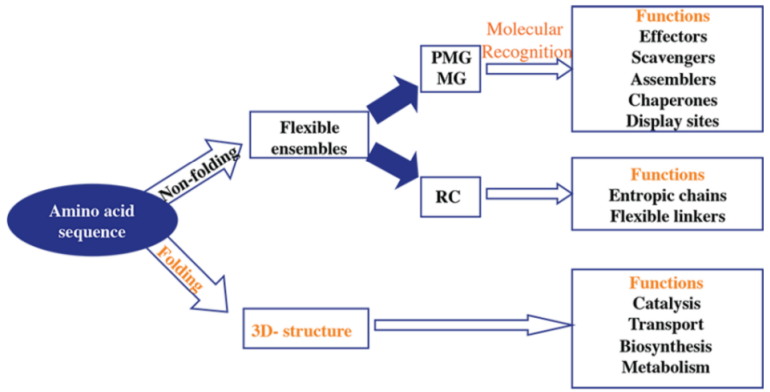
\includegraphics[width=0.9\textwidth]{img/proteinFunctionMechanisms.png} 
% \caption{Distinctive properties of proteins: diversity and functional role. Figura extraida de \cite{habchi2014introducing} }
% \label{proteinMechanisms}
% \end{figure}
% 
% 



\begin{figure}[h!,centered]
\centering
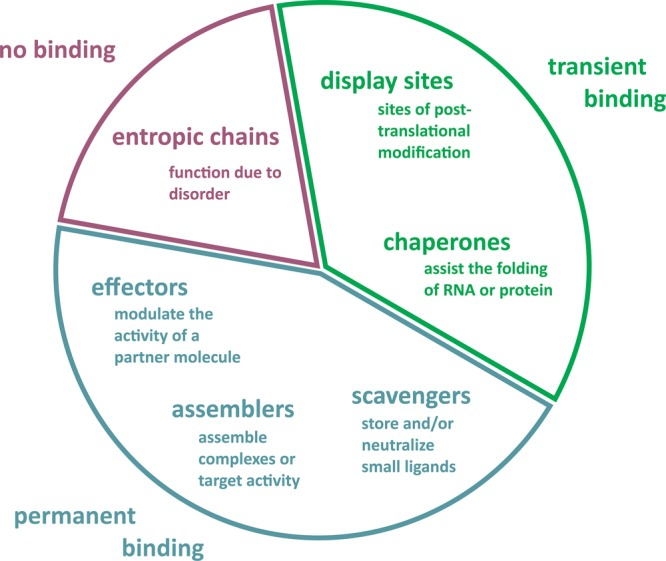
\includegraphics[width=0.7\textwidth]{img/idpFunctionMechanisms.jpg} 
\caption{Clasificación roles y mecanismos funcionales de IDPs/IDRs. Figura extraida de \cite{van2014classification}}
\label{idpFunctions}
\end{figure}


% Para el caso de las proteínas globulares, los dominios son los principales módulos estructurales y funcionales.
% A diferencia de esto, la identificación de las regiones/elementos funcionales dentro de IDPs es un area que todavía está en desarrollo y no es fácil realizar una identificación clara ni mucho menos exhaustiva de éstos. 

% Los elementos asociados al proceso de unión y plegamiento forman el primer conjunto de elementos funcionales 
Dentro de estos segmentos podemos identificar a los elemento de reconocimiento(RE=recognition element)\cite{mohan2006analysis,vacic2007characterization,oldfield2005coupled}, los cuales involucran regiones cortas(10-70 aminoácidos de largo) 
con propiedades generalmente anfipáticas, y se caracterízan porque pueden experimentar un proceso plegado y unión(descrito previamente) que permite la interacción con ligandos.  
% Estos REs(o MoREs por el nombre en inglés de Molecular Recognition Elements) pueden, a su vez, subclasificarse de acuerdo a las estructuras secundarias que adoptan en el complejo de unión. % bound state
% Los dos modelos descritos previamente para el proceso de unión y plegamiento (selección de conformación y unión y plegamiento simultáneo) permiten subclasificar aún más estos elementos desde el punto de vista estructural, 
% agregando el concepto de elementos estructurales preformados(PSEs)\cite{fuxreiter2004preformed}. 
% Estos PSEs se corresponden con el modelo de selección de conformaciones, es decir, son regiones intrínsecamente desordenadas que tienen tendencia a formar elementos estructurales transitivos, adquiriendo temporalmente estructuras secundarias.
% Estos elementos pueden tener la capacidad potencial de servir como sitios de unión y quedar estabilizados en el complejo formado.
% Como primeros elementos funcionales identificados a partir de sus propiedades conformacionales dentro de IDPs tenemos, entonces, a los MoREs y PSEs. 
% Esta clasificación no es totalmente excluyente ya que, como se dijo previamente, puede haber elementos que resulten de una combinacion de estos conceptos.
% 

% ACA CONECTO CON SLM
Más allá de estos elementos que fueron descubiertos a partir de análisis estructurales, el mecanismo de reconocimiento ha sido estudiado desde el punto de vista de los patrones secuenciales que los determinan, 
encontrandose elementos en la secuencia caracterizados por presentar interfaces
de interacción muy compactas (los residuos determinantes de la afinidad y especificidad estan contenidos generalmente en unos 3-11 AAs contiguos).
Estos elementos se conocen como motivos lineales o por sus siglas en inglés, LMs, ELMs, SLiMs o MiniMotifs\cite{davey2012attributes}. 
Como resultado del número limitado de contactos para interacciones con ligandos, los SLMs se unen con una afinidad relativa muy baja lo que resulta en una ventaja considerable 
para participar en interacciones transientes, condicionales y  ajustables, que son propias de los procesos regulatorios.

En términos de funcionalidad, se pueden clasificar los SLMs en dos grandes familias: los que actúan como sitios objetivo de modificaciones post-traduccionales(PTM), 
y los que funcionan como ligandos en la formación de complejos de interacción.
% Dado que el conjunto de funcionalidades y propiedades estudiadas en relación a estos motivos lineales en la secuencia se corresponden en gran medida con las funcionalidades principales de IDRs/IDPs, 
En \cite{fuxreiter2007local} se analizaron los perfiles conformacionales de proteínas que contienen instancias de éstos(no solo la conformación del segmento sino también el contexto), concluyendo que, efectivamente, 
suelen encontrarse formando parte de regiones IDRs y por lo tanto forman parte del conjunto de elementos funcionales característicos de IDPs.
Sin embargo, los SLMs se diferencian de los MoREs descritos previamente en que estos últimos dependen de un patrón de desorden en la secuencia(el cual puede ser obtenido con herramientas de predicción de desorden), 
mientras que los SLMs dependen de motivos secuenciales específicos.

El hecho que esten definidos por solo un pequeño segmento de AAs tiene consecuencias relevantes en aspectos biológicos de los SLM.
En particular, claramente resulta muy probable que estos aparezcan o desaparezcan mediante mutaciones. 
Dado que solo se necesitan un número muy limitado de mutaciones para que surgan, estos son propensos a la evolución convergente, lo que facilita la proliferación en distintos lugares del proteoma.
Esto resulta en una fuente de evolución para la red de interacciones ya que se generan interfaces \textit{de novo} en distintas proteínas.
Estas mismas características dinámicas de la secuencia los hace mas difíciles de estudiar que elementos funcionales mas restringidos evolutivamente como los dominios globulares.
Por lo tanto, a pesar de la disponibilidad de miles de secuencias de proteínas, el descubrimiento de motivos contenidos en estas es aún una tarea difícil.

% SI ENCUENTRO REFERENCIA PARA ESTO LO AGREGO !!!
% Las propiedades de funcionalidad altamente dinamicas y la importancia biologica que tienen estos elementos hacen esperable que esten altamente regulados en la celula.






% *************************************************************
% ******    IDD  ********************
% ACA AGREGO OTRO ELEMENTO, LOS DOMINIOS ID, QUE PUEDEN SER OTRA CLASIFICACION
A pesar que las interacciones mediante SLMs suelen ser débiles, transitivas y, posiblemente, tener baja especificidad, pueden originarse interfaces mas especificas y de mayor afinidad si 
se obtiene cooperación de las regiones flanqueantes, si se combinan varios motivos cortos, o si se utilizan dominios desordenados con mayor longitud.
Es relevante decir que las regiones de unión en IDPs suelen corresponderse mas con dominios que con motivos cortos, teniendo longitudes que exceden los 20-30 residuos
\cite{tompa2009close,chen2006conservation,chen2006conservationB}.  
Además de esta longitud característica, tienen distintas propiedades que los distinguen como dominios:
Son estructuralmente y funcionalmente independientes dentro de la proteína, pueden ser más facilmente reconocibles mediante similitud secuencial debido a que sus secuencias están conservadas, 
y poseen al menos una función específica que los identifica.
Al poder distinguirlos como dominios intrínsecamente desordenados(IDDs) podemos clasificarlos, entonces, como una nueva clase de elementos funcionales independientes que pueden encontrarse dentro de IDPs.
Estos elementos tienen funciones muy diversas pero, generalmente, están involucrados en procesos de interacción con DNA, RNA u otras proteínas.









% 
% % COMENTARIOS APARTE SOBRE LA REGULACION DE IDPs EN LA CELULA
% En términos biológicos las diferencias secuenciales entre las IDRs/IDPs y los segmentos o proteínas totalmente plegadas, además de las diferencias conformacionales antes vistas(y de las diferencias funcionales que veremos), 
% indican que se tratan de entidades separadas dentro del complejo perfil del proteínas naturales existentes.
% Esta claro, además, que no sólo son un elemento real y distinguible, sino que son abundantes en el proteoma, tienen propiedades muy diversas y cumplen funciones vitales para cualquier sistema biológico.
% Todas estas propiedades hacen que parezca razonable que este tipo de proteínas este altamente regulada dentro de la célula \cite{gsponer2008tight,habchi2014introducing}.






% ACTIVIDADES BIOLOGICAS
% 
% Certain biological functions, such as enzyme cat-
% alysis, immunological recognition, or molecular
% discrimination by receptors, absolutely demand
% exquisite control of three-dimensional structure. In
% contrast, functions such as signaling can be
% achieved by linear sequences, simple sequence pat-
% terns, or by isolated secondary structural motifs.
% Intrinsically unstructured proteins, which are
% induced to fold by interactions with other mol-
% ecules, offer several important advantages in sys-
% tems involved in cellular signaling and regulation.
% Unstructured proteins are inherently  ̄exible and
% both their local and global structures can easily be
% shaped by their environment. Such intrinsic plas-
% ticity could allow a single protein to recognize a
% large number of biological targets without sacri®-
% cing speci®city.
% 





























\subsubsection{Agregados proteicos}


% CONCEPTOS GENERALES 

% Las proteínas plegadas, como las proteínas globulares vistas previamente dependen de la estructura  para poder funcionar correctamente, deban atravesar un proceso de plegamiento el cual ocurre, en condiciones normales, de manera muy rápida. 
% Para que los dominios globulares adquieran 
% Esto es posible ya que sus secuencias han evolucionado de forma tal que son capaces de alcanzar la estructura nativa(funcional) muy eficientemente, incluso en el complejo entorno celular.
% Sin embargo, a medida que el tamaño de la proteína aumenta, tambien aumenta la complejidad del proceso de plegamiento y este se vuelve propenso a errores,
% lo que puede llevar a estas proteínas a adoptar conformaciones incorrectas(\textit{misfolded}). 
% Los errores durante este proceso en el que se buscan las interacciones ``correctas'' entre los residuos pueden estar asociados a distintos factores(principalmente mutaciones), 
% no sólo al tamaño de la proteína, ya que de por si el proceso de plegamiento es complejo. 
% Por otro lado, si estos estados estructurales incorrectos mantienen su solubilidad pueden comenzar a acumularse en el entorno celular.
% 
% Ademas de estos estados \textit{misfolded}, algunos intermediarios en el proceso de plegamiento pueden tener tiempos de vida considerables, poblando estados alternativos al plegamiento final.
% Más alla de esto, una vez alcanzada la estructura final, diversas condiciones del entorno pueden producir que este se pierda y se adopte un estado no-plegado(\textit{unfolded}).
% Las proteinas plegadas, entonces, no siempre se encuentran en su estado nativo dentro del entorno celular y pueden ocurrir acumulaciones de estados \textit{misfolded} los cuales, por definición, 
% abarcan a cualquier proteína que no esté en su estado nativo.
% 
% Además del efecto que tiene adoptar un estado \textit{misfolded} sobre la función de la proteína, estos estados pueden también llevar a la formación de agregados entre proteínas
% lo cual tiene, generalmente, un efecto devastador en la célula/organismo.
% A pesar que hemos utilizado el concepto de \textit{misfolding} para introducir la problemática de agregación, estos dos procesos no son necesariamente dependientes entre si, y los agregados representan componentes proteicos mucho 
% mas complejos que la simple acumulación de estados no-nativos, pudiendose originar a partir de diversos estados iniciales mediante procesos que aún hoy son sujeto de estudios, resultando en conformaciones estructurales muy diversas.
% Como se verá, la habilidad de una proteína a formar distintos tipos de agregados depende de muchos factores, entre los cuales están claramente la secuencia y el entorno en que se encuentra,
% de otra forma, las proteinas que adquieran conformaciones no estructuradas o que se encuentren en estados de plegamiento intermedios semi-estables tendrían una tendencia mucho mayor a la agregación y, sin embargo, esto no es así. 

En términos generales, los agregados proteicos se forman por la asociación(interacción) anormal entre proteínas, dando complejos con distintas propiedades y que pueden acumular una gran cantidad de proteínas.
Si bien algunos agregados pequeños pueden mantenerse en solución, en general terminan formando precipitados en condiciones fisiológicas. 

A partir de las características morfológicas de estos, se pueden distingir escencialmente dos tipos: agregados amorfos y fibrillas amiloides.
Los primeros muestran una apariencia granular y consisten principalmente de proteínas en conformaciones desplegadas, aunque presentan ciertas regiones cierto enriquecimiento de estructuras de hoja-$\beta$ plegada, las cuales
mantiene las proteínas unidas formando el agregado.
Por otro lado, las fibrillas amiloides poseen estructuras altamente ordenadas y repetitivas donde todos los polipéptidos que la componen adoptan un plegamiento en común.
% Si bien no nos vamos a enfocar en los detalles puntuales de la estructura, se sabe que 
Estas diferencias que se ven en la conformación macromolecular son el reflejo de diferencias en las interacciones y arquitectura a nivel atómico.
Por otro lado, las diferencias estructurales también se reflejan a nivel biológico: los distintos tipos de agregados tienen afinidades diferentes frente al conjunto de chaperonas y, además, 
pueden acumularse en diferentes localizaciones celulares y ser degradados por mecanismos diferentes.
% Por último, a diferencia de los agregados amorfos, las propiedades únicas de las fibrillasas amiloides han sido aprovechadas por 
% distintos sistemas biológicos y pueden encontrarse versiones funcionales de éstas en distintos organismos\cite{fowler2007functional}.

A pesar que podría parecer obvio, es importante diferenciar los precipitados en los que las proteínas mantienen su estructura nativa de estos agregados que surgen a partir de nuevas estructuras no-nativas.
La precipitación es generada por la inducción de un entorno de solubilidad reducida, por ejemplo durante la precipitación isoeléctrica o mediante sulfato de amonio,
que son los procesos típicos para obtener los cristales utilizados en la resolución de estructuras por difracción de rayos X. 
En estos casos, la reducción de la fuerza iónica o el cambio en el pH de la solución restituye los precipitados a la forma soluble.
El segundo tipo de estructuras macromoleculares representa la formación de interacciones entre proteínas(principalmente formando hojas-$\beta$) que llevan a la formación de estados muy estables, 
reflejados en un profundo mínimo sobre el perfil de energía correspondiente. 
Esto hace que solo sea posible restituir la forma soluble de los componentes mediante procedimientos extremos aunque, igualmente, es dificil que las proteínas vuelvan a adoptar sus conformaciones nativas.
% permanenciendo en solución aconformaciones mal plegadas.
Este tipo de agregados es de nuestro mayor interés en el trabajo ya que puede ocurrir en condiciones experimentales ``normales'', que no han sido inducidas con el fin de formarlos.


En el gráfico \ref{aggregationDiagram} se muestran distontos agregados proteícos, integrados dentro del perfil conformacional de las proteínas, mostrando los distintos tipos de estructuras de agregación, 
los intermediarios a partir de los cuales se originan, y los equilibrios y mecanismos para desintegrarlos. 


\begin{figure}[h!,centered]
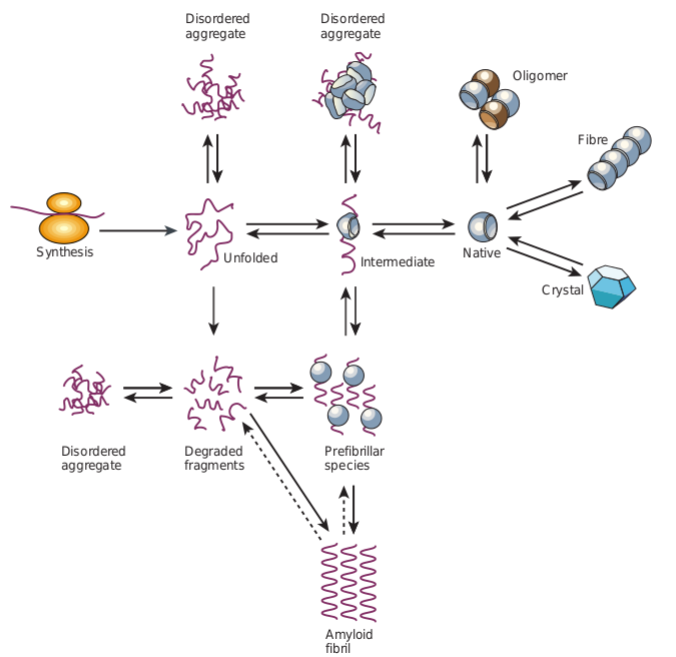
\includegraphics[width=\textwidth]{img/aggregationDiagram.png} 
\caption{} \label{aggregationDiagram}
\end{figure}



% ESTRUCTURA
Las fibrillas amiloides son, probablemente, el tipo de agregado más interesante y el más estudiado, ya que tiene propiedades que las hacen muy particulares.
En primer lugar, como se mencionó antes, adoptan estructuras altamente ordenadas y compactas, similares en parte a los estados nativos de proteinas globulares.
Por otro lado, parte de las propiedades únicas de este tipo de estructuras es que, probablemente debido a su estructura de puentes de hidrógeno altamente organizada, posee una estabilidad cinética única.
Por lo tanto, una vez formados estos agregados pueden mantenerse durante largos períodos de tiempo, funcionando como núcleo para la agregación de más cantidades de la misma proteína 
y permitiendo la formación de depósitos en la célula/tejido.

La formación de agregados amiloides fue observada por primera vez en el contexto de la amiloidosis sistémica hace mas de 150 años y, de hecho, obtuvo su nombre en este descubrimiento cuando se encontró que 
los depósitos observados respondían a la tinción con iodo, el colorante usado para la deteccion de almidón. 
Desde entonces, se encontró que los depósitos de proteínas encontrados en distintas enfermedades provocadas por \textit{misfolding} de proteínas poseían estas características amiloides.
Estos depósitos estaban conformados generalmente de un solo tipo de proteínas, aunque se encontraban \textit{in-vivo} asociados a distintas moléculas.
Los estudios más avanzados de su estructura revelaron las características altamente ordenadas, compactas, estables y no-ramificadas que poseen estos agregados y que se ven reflejados en
la morfología fibrilar que puede apreciarse al verlos mediante el microscopio electrónico de transmisión.
El diámetro de estas estructuras fibrilares(fibrillas) se encuentra en el rango de los 10 \textit{nm} y su longitud puede alcanzar varios micrómetros. 
Estas fibrillas maduras pueden, además, asociarse lateralmente entre si para formar fibras.

Todas las fibrillas amiloides comparten una arquitectura en común compuesta de una estructura suprasecundaria de unión entre hojas-$\beta$.
Los detalles de esta arquitectura, obtenidos mediante difracción con rayos X, revelan que 
las hojas-$\beta$ se extienden con las caras de sus hebras enfrentadas entre si pero perpendiculares al eje de la fibrilla que forman\cite{nelson2005structure}.  
Esta arquitectura de hojas-$\beta$ cruzadas permite, como se mencionó antes, la formación de un continuo de puentes de hidrógeno que provee a estas componentes de gran estabilidad. 
En la figura \ref{amyloidStructure} se ve una representación gráfica detallada de esta estructura.



\begin{figure}[ht]
\centering
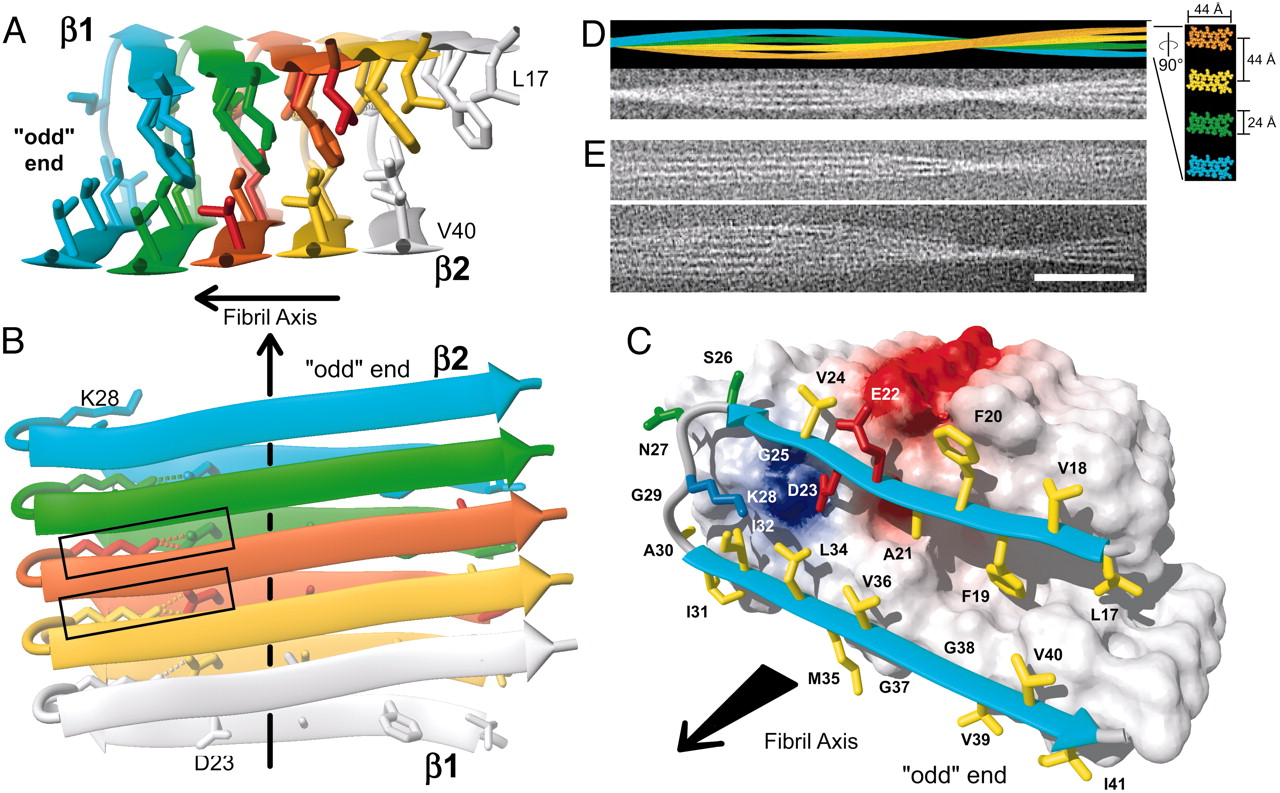
\includegraphics[width=0.9\textwidth]{img/amyloidStructure.jpg} 
\caption{Estructura de fibrillas amiloides. Figura extraída de \cite{luhrs20053d}}
\label{amyloidStructure}
\end{figure}



% SACO TODA LA PARTE DEL PERFIL ENERGETICO
% ******************************************
% ENERGY LANDSCAPE
% 
% En la figura \ref{fullEnLandscape} se muestra la representación gráfica de la estabilidad termodinámica resultante, junto a otras estructuras posibles.
% Los complejos funcionales que se forman entre IDRs/IDPs y sus ligandos implican la formación de nuevas interacciones intermoleculares que cambian el perfil energético del ensamble,
% creando estados de mínima energía claramente definidos con características estructurales propias.
% Mediante un mecanismo similar, la interacción entre proteínas lleva a la formación de distintos estados agregados generalmente no-funcionales(oligómeros, agregados amorfos, fibrillas amiloides, etc.).  
% En este caso, las interacciones llevan a la formación de estados muy estables, reflejados en un profundo mínimo sobre el perfil de energía correspondiente. 
% 
% 
% \begin{figure}[ht!]
% \centering
% \begin{subfigure}[ht]{\linewidth}
% 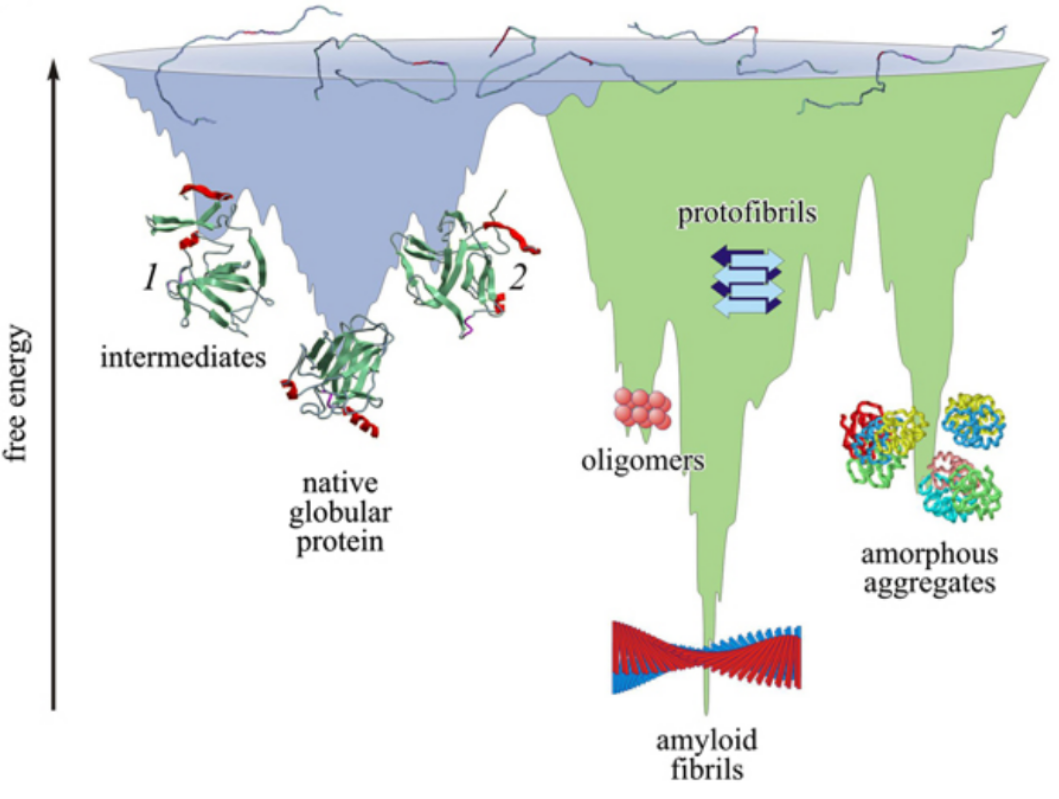
\includegraphics[width=0.7\textwidth]{img/globularEnLandscape.png} 
% \centering
% % 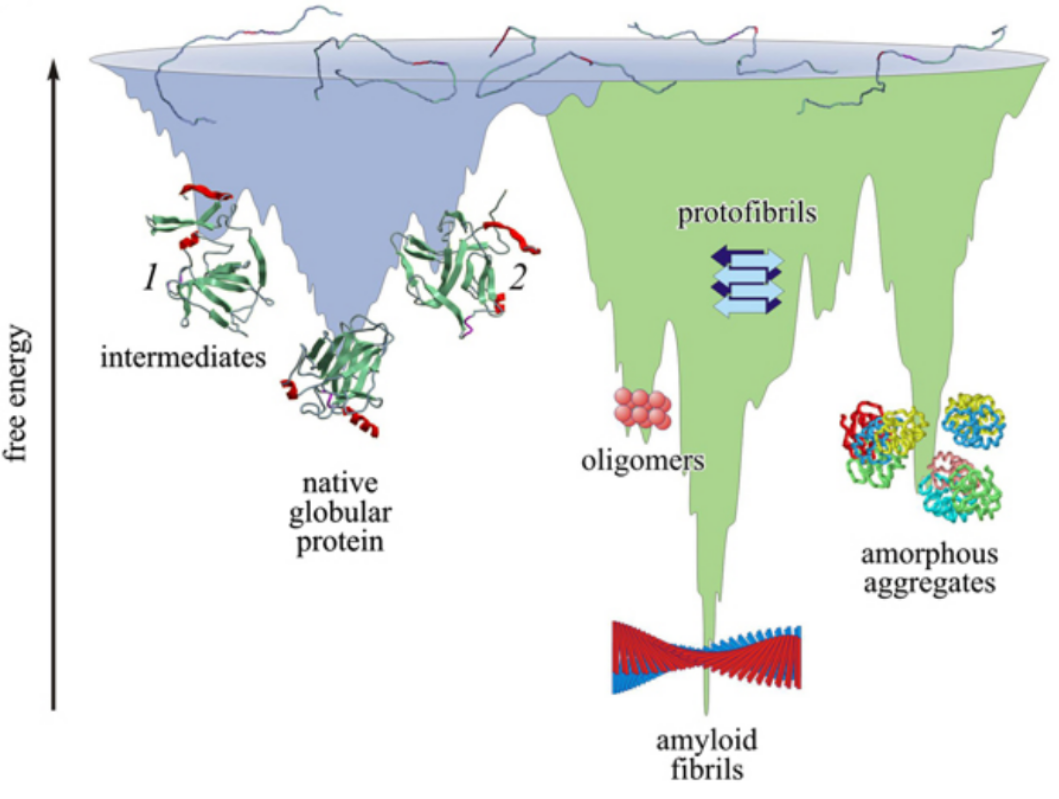
\includegraphics[width=0.7\textwidth]{img/globularEnLandscape.png} 
% \caption{Perfil energetico de los estados de un polipeptido con estructura nativa globular. Figura extraida de \cite{turoverov2010protein}}
% \label{globularFullEnLandscape}
% \end{subfigure}
% 
% \begin{subfigure}[ht]{\linewidth}
% \centering
% 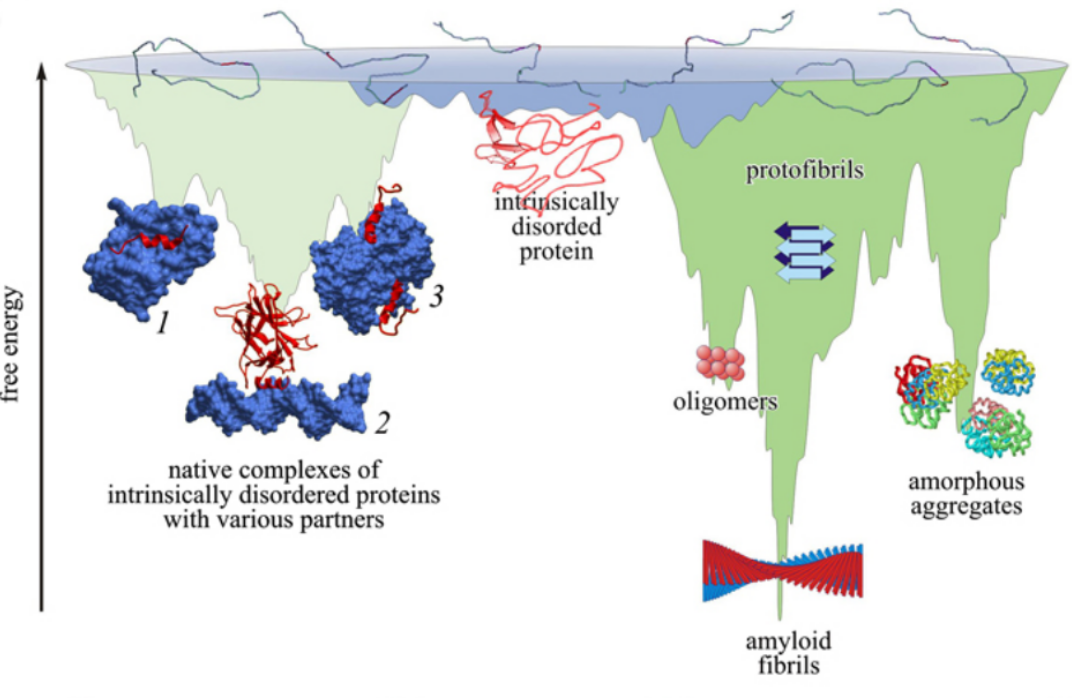
\includegraphics[width=0.7\textwidth]{img/idpEnLandscape.png} 
% \caption{Perfil energetico de los estados de un polipeptido con estructura nativa desordenada. Figura extraida de \cite{turoverov2010protein}}
% \label{idpFullEnLandscape}
% \end{subfigure}
%  \caption{Full energy landscape}
%  \label{fullEnLandscape}
% \end{figure}
% 
% 
% 
% 
% Como se ve en la fig.\ref{fullEnLandscape}\textbf{(a)}, en condiciones normales, donde los proteínas se mantienen en sus estados plegados, 
% la estabilidad de estos estados los mantiene separados mediante barreras cinéticas relativamente altas de la formación de agregados(que se muestran considerablemente mas estables).
% Esto no es tan determinante para intermediarios del plegamiento(estados 1 y 2 en fig. \ref{fullEnLandscape}\textbf{(a)}) y para las conformaciones desplegadas(fig. \ref{fullEnLandscape}\textbf{(b)}), 
% donde las barreras energéticas pueden no ser determinantes en el mantenimiento de los estados nativos en solución.
% Teniendo en cuenta que, como vimos antes, existe una gran diversidad de estados conformacionales en la célula,que el estado totalmente ordenado es, quizás, solo una excepción, 
% y además se sabe que los agregados pueden provocar un gran daño biológico,
% es esperable que los sistemas biológicos hayan evolucionado distintos mecanismos para mantener la homeostasis de los estados nativos monoméricos.
% 







% PROPIEDADES SECUENCIALES
A pesar de esta arquitectura claramente definida de las fibrillas amiloides, las proteínas que forman estos agregados son muy diversas, con muy poca similitud entre sus secuencias.
% o sus conformaciones monoméricas en solución.
Lo que es más relevante, estudios con diversos péptidos y proteínas (no relacionados con aquellos encontrados como causantes de la amiloidosis sistémica) muestran que todos son capaces de formar, 
bajo las condiciones apropiadas, agregados con las características de las fibrillas amiloides.
Estos estudios experimentales, junto con una gran variedad de analisis computacionales, llevan a pensar que la estructura amiloide puede ser adoptada por cualquier cadena polipeptídica y, por lo tanto, 
esta habilidad para reordenar la conformación monomérica y agregarse para formar la estructura amiloide característica puede ser una propiedad intrínseca de las proteínas\cite{fandrich2002behaviour}.
El estado estructural amiloide parece ser, entonces, un estado generico de las proteinas.

Sin  embargo, la tendencia a formar este tipo de fibrillas amiloides si es un proceso que depende específicamente de la secuencia, y algunos detalles estructurales a nivel atómico, 
así como la estabilidad relativa del estado amiloide, pueden ser también características fuertemente dependientes de la secuencia. %REFERENCIAS????  
Por lo tanto, la tendencia a formar estos estados agregados puede variar ampliamente entre distintas proteínas, la pregunta clave es ¿cómo influye la secuencia(o composición) de aminoácidos sobre esta tendencia?
La respuesta a esto es importante no sólo para entender los estados de agregación y sus mecanismos de formación, sino también para otros aspectos como 
la producción biotecnológica de proteínas, o el diseño racional de cadenas polipeptídicas funcionales, donde se desea evitar la formación de agregados al (sobre)expresar las proteínas.
Estos conocimientos sirven también como base para el desarrollo de herramientas bioinformáticas que permitan detectar la tendencia a formación de agregados a partir de una secuencia.

% DEPENDENCIA CON LA COMPOSICION
Se sabe que las interacciones hidrofóbicas son esenciales para la compactación de la estructura lineal de un polipéptido.
Se podría esperar, entonces, que un incremento en el contenido de residuos hidrofóbicos pueda aumentar la tendencia a la agregación de una secuencia, mientras que un incremento en la carga neta impida esta agregación. 
Además de estas propiedades fisicoquimicas, dadas las características estructurales recién descritas para las fibrillas amiloides, con un alto contenido de hojas-$\beta$, 
es razonable pensar que las secuencias que tienen una tendencia intrínseca a adoptar conformaciones de hoja-$\beta$ en su estructura secundaria probablemente tendrán, también, cierta tendencia a la formación de estos agregados.  
% En \cite{chiti2003rationalization} se estudian todas estas propiedades secuenciales mediante mutaciones sistemáticas sobre polipéptidos, concluyendo 
% que la estructura primaria de un polipéptido cumple un papel muy importante en la tendencia a formar depósitos insolubles.


% DEPENDENCIA CON SEGMENTOS DE SECUENCIA
La composición secuencial parece tener un papel importante en la tendencia a la agregación, sin embargo, la combinación lineal de estas propiedades a lo largo de la estructura
primaria puede tener un impacto aún mayor, es decir, no todas las secuencias de polipéptidos con la misma composición tienen la misma tendencia a la agregación.
En \cite{ventura2004short} se demuestran la existencia de ciertos tramos cortos en la secuencia que promueven la agregación en estructuras amiloides.
Estos tramos cortos, llamados generamente regiones propensas a la agregacion(o APRs) se distinguen por tener composiciónes características de residuos, ricas en residuos hidrofóbicos.
% The analysis of the structural models for some amyloids also allow to rationalize the reason why APRs direct the formation of amyloid-like structures, since the cross-$\beta$ arrangement in the core of
% amyloid fibrils does only strictly require the minimum participation of a single $\beta$-strand per molecule, and the rest of the polypeptide may remain exposed to the
% solvent even when “attached” along the fibril.

% ESTO DE LAS REGIONES PEQUEÑAS LO TENGO QUE PONER PORQUE ES LA BASE DE ALGUNOS METODOS QUE DESPUES USAMOS
Además del análisis secuencial, existen otras evidencias a favor de la hipótesis que algunas regiones pequeñas de las proteínas son responsables principales de la formación de fibrillas amiloides. 
Por ejemplo, la mayoría de las IDPs no experimentan agregación \textit{in-vivo}\cite{linding2004comparative} lo que indica que, si bien la conformación no-plegada es necesaria, no es condición suficiente 
para promover el proceso de agregación.
Por lo tanto, deberían existir patrones secuenciales distinguibles que, una vez expuestos(salen del núcleo hidrofóbico de la estructura plegada), son mas propensos a la agregación que otros.  

El hecho que en la naturaleza las IDRs/IDPs no sean necesariamente propensas a la agregación implica, entonces, que sus secuencias han evolucionado para mantener el nivel de solubilidad necesaria que es requerido para 
realizar correctamente las funciones asociadas, por ejemplo, a través de extensas regiones de aminoácidos con grupos polares y altamente cargados que desestabilizan las asociaciones intermoleculares.
Hay que destacar, sin embargo, que existen barreras cinéticas que ayudan a los sistemas biológicos a mantener tanto las IDRs/IDPs como las proteínas plegadas en solución, evitando la formación de agregados no-funcionales 
y manteniendo la homeostasis de los estados proteícos.

% FACTORES EXTERNOS QUE AFECTAN LA AGREGACION
Además de las propiedades que se analizaron sobre la secuencia primaria, es importante destacar factores externos a la secuencia que pueden afectar la formación de agregados.
Los determinantes extrínsecos mas relevantes son el pH y la fuerza iónica de la solución, junto con la temperatura del sistema.
Estas variables pueden afectar tanto la cinética como las propiedades termodinámicas de los diferentes estados e intercambios entre estos.
Estas propiedades afectan a todos los estados posibles aunque en este caso los mencionamos en el contexto de proceso de agregación.





% ACTIVIDADES
Los agregados proteícos estan generalmente asociados con condiciones anormales donde se pierde la capacidad de mantener las proteínas en sus estados nativos correspondientes(pérdida de homeostasis proteica) y, por lo tanto, 
se pierda la capacidad de estas para realizar sus actividades biológicas(al menos de forma correcta) con las obvias consecuencias negativas para el sistema. 
En particular las fibrillas amiloides fueron descubiertas en el contexto de una enfermedad sistémica y se cree que están asociadas a una gran cantidad de enfermedades, sin embargo,
han sido aprovechadas por distintos sistemas biológicos y pueden encontrarse versiones funcionales de estos agregados en distintos organismos\cite{fowler2007functional}.





% % FUNCTIONAL AMYLOIDS
% Amyloids are not only associated with disease-related proteins.
% Nature also exploits the structural and mechanical properties
% of amyloids to regulate biological functions 13 . For example, in
% bacteria amyloids such as curli promote biofilm formation and
% host invasion, and chaplins in bacteria and hydrophobins in yeast
% act as regulators of surface tension of water. Insects and fish
% use chorion amyloid as a component of eggshell, and spiders
% use spidroins in spider silk. Humans possess at least one func-
% tional amyloid protein: Pmel17 is used as a structural scaffold
% in melanin synthesis. The strength and flexibility of amyloids
% have attracted attention for their use as biomaterials. However,
% it remains to be understood how functional amyloids avoid the
% cytotoxic effects observed in disease amyloids. In part, functional
% amyloids are regulated by chaperones and proteases. But it is
% also becoming evident that sequence composition modulates
% critical biophysical parameters determining kinetics of assembly
% or mechanical strength.






% Las fibras amiloides se consideran que estan asociadas to more than 40 human pathologies, esto generó un gran interés en estudiar sus propiedades, 
% las formas detectar secuencias con tendencia a formarse y las formas de prevenir su formación in vivo.


% Since all fibrils independent of the original structure of the given amyloidogenic protein have a common cross-b structure, considerable conformational rearrangements have to occur prior to fibrillation. 
% Such changes cannot happen in a native protein, due to its stable and rigid tertiary structure. Thus, protein destabilization favoring partial unfolding and culminating in the formation of a partially unfolded conformation is required. 
% Presumably, such a partially unfolded conformation favors reciprocal and specific intermolecular interactions, including electrostatic attraction, hydrogen bonding and hydrophobic contacts, which are necessary for oligomerization and fibrillation
% Obviously, this model does take into account a class of natively unfolded proteins, as they are devoid of rigid tertiary structure in their native state.

% Data have been reported indicating that the first critical step in protein fibrillogenesis is the partial unfolding of the protein. 
% Due to structural fluctuations (conformational breathing) the structure of a globular protein under physiological conditions represents a mixture of tightly folded and multiple partially unfolded conformations, 
% with great prevalence of the former. 
% Most mutations associated with accelerated fibrillation and protein deposition diseases have been shown to destabilize the native structure, increasing the steady-state concentration of partially folded conformers

% En la mayoria de las proteinas, excepto las mas pequeñas, el 'unfolding' que ocurre en condiciones fisiologicas no lleva a una estructura totalmente desplegada sino que la proteina adquiere una estructura semi-estable parcialmente collapsada,
% donde las interacciones no son las mismas que en el estado nativo estructurado, estas son caracteristicas propias de los intermediarios del plegamiento.

% The energy landscape model suggests that some folding intermediates might have structural elements not present in the final folded state(en el estado final pueden estar metidas en el centro hidrofobico).
% The appearance of such misfolded intermediates might initiate protein oligomerization or aggregation.

% La formacion de estos intermediarios es importante porque generalmente son mucho mas solubles que si se formaran conformaciones altamente desplegadas. 
% Esta solubilidad permite alcanzar las concentraciones requeridas para la nucleacion propia de la formacion de amyloids(y de agregados en general????)

% Detailed structural analysis of early fibrillation events in several proteins has demonstrated that the amyloidogenic conformation is only slightly folded and shares many structural properties with the premolten globule state.

% This picture enables us to speculate on the origins of the amyloid diseases from the point of view of the physico-chemical properties of the protein molecules. 
% If the stability or cooperativity of the native state of a protein is reduced, for example by a mutation, the population of non-native states will increase.
% This rise will increase the probability of aggregation, as the concentration of polypeptide chains with at least partial exposure to the external environment will be greater. 


% La ocurrencia o no de la formación de agregados dependerá, entonces, de la tendencia intrínseca que posee la secuencia, de la concentración de proteínas y del proceso de agregación.
% Sin embargo, a pesar de la diversidad de estudios al respecto, no se tiene aún conocimiento del mecanismo molecular subyacente a la transformación de proteínas solubles en agregados amiloides.
% % Despite active research, a detailed understanding of the molecular principles underlying the transformation of soluble proteins into amyloid aggregates is still lacking
% % Whether or not aggregation does occur will depend on the concentration of protein molecules, the intrinsic propensity for a given sequence to aggregate when unfolded, and on the rate of the aggregation process. 
% Se ha encontrado que la formacion de fibrillas amiloides puede ser generado utilizando un nucleo estructural como en los procesos de cristalización.
% % The fact that formation of ordered amyloid fibrils can be seeded, like the well-studied processes of crystallization and gelation,
% Esto parece indicar que, una vez iniciado el proceso de agregación, este avanza muy rapidamente en la acumulación y expansión.
% % means that once the aggregation process is initiated it often proceeds very much more rapidly.

% In the absence of seeding there can be long 'lag' phases before aggregation occurs . 
% This lag can be thought of as arising because the growth of a fibril cannot occur until a 'nucleus' of a small number of aggregated molecules is formed. 
% Such a nucleus can be formed by the local fluctuations in concentration that occur in solution as a result of random molecular motion. 
% When such fluctuations result in a local concentration of molecules above a critical value, the molecules associate with one other to form a species that is suficiently 
% large to have intrinsic stability, and hence to grow in size by interacting with other molecules in the solution. The act
% of seeding provides such nuclei to the solution and hence reduces or abolishes the lag phase
% 
% The proposal that amyloid fibrils are a generic structure of polypeptide chains (lo que los hace genericos, que se desarrollo antes) coincide con este modelo de formación.







% 
% The prion protein, for example, is
% thought to undergo a conformational transition
% from a normal cellular form containing a prepon-
% derance of helical secondary structure to a plaque-
% forming conformer containing a greater proportion
% of b-sheet (Pan et al., 1993). Structure determination
% of fragments of the prion protein (Riek et al., 1996;
% James et al., 1997) revealed that  aprox.100 residues at
% the C terminus are folded into a largely helical
% domain. Somewhat surprisingly, NMR studies of
% the full-length protein (aprox200 residues) indicated
% that the N-terminal half of the protein is completely
% unfolded under normal solution conditions (Donne
% et al., 1997). Partial folding of a local region contain-
% ing four octapeptide repeats occurs in the presence
% of Cu(II) ions (Viles et al., 1999) and may give a clue
% as to the overall physiological function of the prion
% protein, which is at present unknown. If this protein
% functions as a copper storage or transport protein,
% the extreme  ̄flexibility of the N terminus is probably
% of functional signi®cance, as the membrane-
% anchored protein picks up copper ions from the
% extracellular fluid.





























\subsubsection{Continuo resultante de estructuras, secuencias y actividades}

Al estudiar las propiedades conformacionales de las proteínas intentamos clasificar los conocimientos en distintos elementos estructurales(proteínas globulares, intrínsecamente desordenadas, etc), esto sirve como modelo para
entender y predecir las propiedades de interé(conformacionales y funcionales principalmente).
La realidad es que, como se dijo en la primera sección de este capítulo, la ocurrencia de proteínas está ajustada a los requerimientos del sistema y al mecanismo evolutivo subyacente, por lo tanto, 
incluso si tratamos de agruparlas en clases distintas, el perfil de muchas propiedades asociadas a las proteínas muestran un perfil que es mejor descrito mediante un continuo de posibilidades.

Ejemplo de esto es el perfil de propiedades conformacionales encontrados en las proteínas. 
A pesar que intentamos distinguir perfiles conformacionales con estructuras tridimensionales definidas(y propiedades dinámicas reducidas), de aquellas que no adoptaban una estructura ordenada, 
el perfil conformacional real que se observa en el proteoma forma un continuo estructural similar al que se ve en la figura \ref{conformationContinuum}.
El extremo izquierdo representa el perfil de las proteinas completamente plegadas. 
En \cite{gall2007intrinsic} se ve que, incluso en la PDB donde las estructuras almacenadas están sesgadas hacia el perfil de proteínas plegadas(porque son las más simples para cristalizar), las conformaciones totalmente ordenadas son 
poco abundantes y que la mayoría de las estructuras posee al menos un segmento desordenado.
Este y otros estudios parecen indicar que el comportamiento de las proteinas totalmente plegadas es la excepción más que la regla, y que la mayoria de las secuencias tienen regiones desordenadas, por lo tanto las estructuras encontradas 
en el proteoma se expanden hacia la derecha del gráfico hasta llegar a un perfil conformacional que no muestra nivel de ordenación estructural a lo largo de su secuencia.


\begin{figure}[htbp]
\centering

\includegraphics[width=1.0\textwidth]{img/conformationContinuum.png} 
\caption{ Continuo estructural: Los segmentos desordenados pueden comprender solo un pequeño conjunto de aminoácidos dentro de las proteínas u ocupar grandes segmentos de ésta, resultando en un
perfil similar al que se ve en la figura. De izq. a derecha: estructura totalmente ordenada; extremos N y C terminales desordenados; región linker desordenada uniendo dominios globulares; loop desordenado;
dominio completamente desordenado; proteína desordenada con elementos estructurales residuales; proteína desordenada sin elementos estructurales definidos pero con conformación colapsada; proteína totalmente desordenada.
}
\label{conformationContinuum}
\end{figure}






% SACO TODA LA PARTE DE PERFIL ENERGETICO
% 
% DIFERENCIAS EN EL PERFIL DE ENERGIA LIBRE
% Todo lo descrito previamente acerca de proteínas plegadas, sus diferencias con el perfil de las IDRs/IDPs, y la estabilidad de los distintas conformaciones del ensamble, 
% puede entenderse mejor si se analizan las superficies de energía libre asociadas. 
% En la figura \ref{idp-folded-EnergyLandscape} se ven ejemplos de estos paisajes energéticos para tres ejemplos representativos de todo el continuo de conformaciones vistas.
% 
% El gráfico que se ve en la figura \ref{idp-folded-EnergyLandscape}\textbf{(a)} muestra el perfil de energía libre frente a los cambios conformacionales asociados para una proteína plegada.
% El perfil con la forma similar a un embudo, característico de este tipo de proteínas, representa lo que se describió previamente sobre éstas, a través del plegamiento alcanzan una estructura ``única'' que 
% representa el mínimo global de energía. 
% Como detallamos, esta estructura única representa en realidad un ensamble de conformaciones con muy pocas variaciones, capaz de ser representado por una estructura promedio.
% Diversos estudios sobre el proceso de plegamiento resultaron en una gran diversidad de teorías sobre los detalles de este paisaje energético y como se relaciona con el proceso de plegamiento.
% Sin embargo, lo mas relevante se obtiene de observar la forma en que se ubican los mínimos de energía y la amplitud de éstos, lo que nos dará una idea del ensamble real que encontraremos en condiciones fisiológicas.
% % Folded proteins have a "funnel-shaped" global free energy minimum, where the lowest energy state corresponds to the 11native structure, and the width of the unique global energy minimum
% % determines the conformational entropy of the native state.
% 
% A medida que nos movemos hacia la derecha en el continuo de conformaciones posibles de la figura \ref{conformationContinuum}, los segmentos desordenados 
% modifican el perfil energético aplanando la superficie en el mínimo global de energía. 
% Este cambio(graficado en la figura \ref{idp-folded-EnergyLandscape}\textbf{(c)}) representa la existencia de nuevas estructuras con una diferencia conformacional considerable con respecto al resto de las estructuras del ensamble, 
% pero que están separadas entre si por barreras energéticas pequeñas. 
% 
% El perfil energético continua aplanándose a medida que aumentan las regiones desordenadas de la proteína.
% En la figura \ref{idp-folded-EnergyLandscape}\textbf{(b)} se ve el perfil 
% correspondiente a una proteína con una conformación completamente desordenada. 
% 
% \begin{figure}[h]
% \centering
% 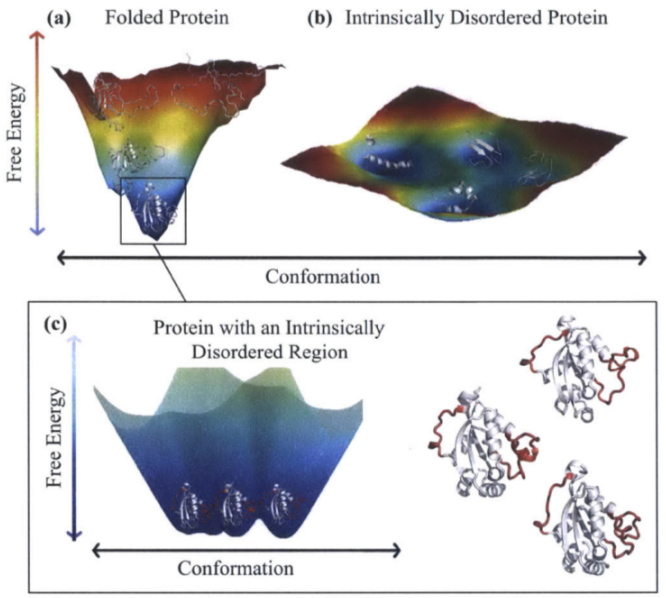
\includegraphics[width=0.7\textwidth]{img/idp-folded-EnLandscape.png} 
% \caption{Diferencias en el paisaje energético entre polipéptidos que adquiren estructuras plegadas, IDRs e IDPs }
% \label{idp-folded-EnergyLandscape}
% \end{figure}










% DIFERENCIAS Y SIMILITUDES ENTRE SLiMs, MoREs e IDD
% 
Algo similar ocurre con los elementos funcionales emergentes de la secuencia.
% A lo largo de las secciones previas vimos diferentes elementos funcionales que, mediante clasificaciones, 
Por ejemplo, como vimos, hay diferencias conceptuales entre los elementos definidos como motivos secuenciales y los MoREs. 
Sin embargo, también existen varias propiedades en común incluyendo la tendencia intrínseca al desorden, ser propensos a experimentar transiciones a estructuras ordenadas y a promover la formación de complejos. 
% Although there are differences in the definitions of linear motifs and MoRFs, they share many common features 72,163 including a tendency to undergo disorder-to-order transition (all
% MoRFs by definition and aprox. 60\% of LMs 48 ), an enrichment in IDRs (MoRFs by definition and aprox. 80\% of LMs are in IDRs 48,72 ), and a tendency to promote complex formation.
Varios estudios sugieren, entonces, que existen un gran solapamiento entre lo que normalmente definimos como motivos lineales y MoREs\cite{fuxreiter2007local,meszaros2012disordered}.
% Yet, interestingly, recent analysis suggests that linear motifs (LMs) (thus not differentiating between ELMs and SLiMs) show high overlap with MoRFs 
Dependiendo si la idea es definida/estudiada desde un punto de vista estructural o secuencial, entonces, un motivo lineal puede ser también identificado como un MoRE o PSE.
Más allá de esto, a pesar de tener una longitud (al parecer) bastante mayor, los IDDs también poseen un solapamiento significativo con MoREs y motivos lineales.
% intrinsically disordered domains (IDDs) can also have significant overlap with MoRFs and linear motifs
Estos resultados parecen indicar que estos elementos funcionales que identificamos con propiedades diferentes pertenecen a estados de un mismo continuo de mecanismos de unión que pueden encontrarse en IDPs.
% The overlap between linear motifs and MoRFs
% especially, but also IDDs, suggests that these functional features
% are different states in the same continuum of binding
% mechanisms involving disordered regions.

% Different concepts regarding short recognition elements have
% been extensively discussed in the literature. Indeed,
% depending
% on whether the idea is approached from a structural point of view
% or defined at the sequence level, a short motif could be denoted
% as a “molecular recognition element” (MoRE)/“molecular
% recognition feature” (MoRF) , a PSE, or “linear motif” (LM),
% respectively (LM is also denoted as “eukaryotic linear motif”
% (ELM) or “short linear motif” (SLiM)).


% ESTO ES LO MISMO, LO COMENTÉ PERO SE PUEDE RESCATAR ALGO
% Whereas LMs have been identified as short sequence motifs critical in recognition functions, primary contact sites, preformed structural elements and molecular recognition elments/features 
% have been approached from the direction of protein disorder, emphasizing recognition segments embedded in such regions. U
% nity of these concepts is underlined by the key role of a few specificity determinants in all these recognition elements, and also by their local preferences 
% for undergoing disorder-to-order transition upon molecular recognition, which might already
% be manifested prior to binding. 
% Apart from a minority of the cases when LMs are constituted of segments of ordered domains, these different concepts of short recognition elements express the same underlying physical and
% functional principles that provide a probably widespread solution to the dynamic control of protein-protein interaction networks.
% 




   
       
       
       

       
%     1.3.1. Ingeniería de proteínas
%         1.3.1.1. Ingeniería de proteínas modulares (a.k.a. quiméricas) (Qué es, 1 página)
%         1.3.1.2. Ejemplos (1 página y 1 figura)
%     1.3.2. Ingeniería de linkers.
%         1.3.2.1. Diseño positivo (propiedades deseadas, 1 página, 1 figura)
%             1.3.2.1.1. Propiedades conformacionales
%             1.3.2.1.2. Carga
%         1.3.2.2. Diseño negativo (propiedades no deseadas, 2 páginas y 1 figura)
%             1.3.2.1.1. Propiedades conformacionales
%             1.3.2.1.2. Propiedades espectroscópicas
%             1.3.2.1.3. Actividades biológicas
%             1.3.2.1.4. Carga metabólica
%         1.3.2.3. Linkers naturales
%             1.3.2.3.1 Características (1 página y 1 figura)
%             1.3.2.3.2 Uso en ingeniería de proteínas (ventajas y desventajas, 1 página)
%         1.3.2.4. Diseño racional
%             1.3.2.4.1 Diseños y conceptos comunes (1 página y 1 figura)
%             1.3.2.4.2 Algoritmos existentes (cómo funcionan, ventajas y desventajas, 2 páginas y 2 figuras)
%             
       
\section{Ingeniería de proteínas}\label{proteinEngineering}
\subsection{Ingeniería de proteínas modulares}    

Como producto de los avances logrados en las tecnologías asociadas al ADN recombinante, se ha desarrollado una nueva generación de proteínas compuestas por la integración
de diferentes módulos secuenciales.

La idea de armar proteínas a partir de la unión de módulos no es algo nuevo, sino que sigue la lógica presentada previamente de que las proteínas naturales son usualmente modulares. 
Es decir, se está simulando el proceso evolutivo natural que desarrolla nuevas proteínas mediante la combinación de dominios preexistentes.

La utilización de la técnica de ADN recombinante para construir nuevas proteínas abre toda una gama de posibilidades que van desde inserción de pequeñas secuencias en extremos de proteína naturales, 
con el fin de poder identificarlas o separarlas, hasta el diseño de construcciones proteicas que buscan obtener nuevas funcionalidades o propiedades diferentes.
% construidas mediante la combinación de distintos dominios.
% En los casos más simples el proceso puede ser ...
% En el caso de nuevos diseños, donde se busca combinar módulos para dar nuevas funcionalidades o hacerlas más eficientes, el proceso experimental puede ser mas complejo.

% s primeros ejemplos de construcciones artificiales probablemente sean la inserción de epítopes o tags(pequeñas secuencias?) en los extremos de alguna proteína para poder localizarlas y/o separarlas.
% en solución o en el entorno celular.
% Más adelante se desarrollaron nuevas construcciones combinando unidades estructurales y/o funcionales en una sola molécula. 
% Esta fusión de dos o más dominios abre toda una gama de posibilidades para construir proteínas con nuevas o mejores funcionalidades.
% 

% Las distintas bases de datos permiten obtener, entonces, una gran cantidad de módulos estructurales y funcionales y gran parte del diseño de proteínas quiméricas 
% se basa en utilizar estos conocimientos y anotaciones para crear nuevas proteínas con estructuras/funciones/propiedades combinadas.

En estos últimos casos, la implementación del proceso experimental suele ser más complejo, requiriendo varios aspectos de diseño a considerar, los 
los cuales no siempre son totalmente independientes entre si. 
% requiriendo un diseño   o un proceso iterativo.
Por un lado está el proceso de diseño/construcción de la nueva proteína.
Por otro están los aspectos asociados con la técnica de ADN recombinante y expresión de proteinas heterólogas. 
En el gráfico \ref{esquemaProcesoFusion} se representan los pasos generales que pueden formar parte de este proceso.

\begin{figure}[htbp]
\centering
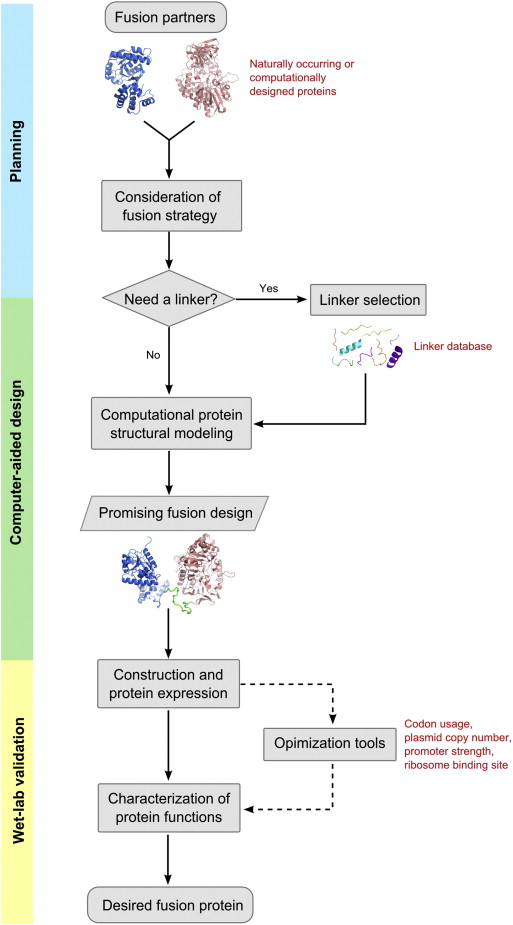
\includegraphics[width=0.7\textwidth]{img/esquemaProcesoFusion.jpg} 
\caption{Figura obtenida de \cite{yu2015synthetic}}
\label{esquemaProcesoFusion}
\end{figure}

La construcción de la proteína de fusión(quimérica) requiere, por su parte, de dos elementos indispensables: 
los dominios o proteínas a fusionar, y la secuencia linker que los va a unir.
La elección de los dominios/proteínas está fuertemente ligada al producto final que se desea obtener y, normalmente, es una decisión directa alrededor de la cual se diseña el resto del experimento.
Por otro lado, la selección de un linker adecuado para unir los dominios/proteinas de acuerdo al objetivo que se busca puede ser un paso complicado y es generalmente ignorado cuando se piensa en el diseño de una proteína quimérica.
La unión directa de los dominios/proteínas o el uso de un linker inadecuado puede resultar en resultados indeseables, por ej. puede restringirse la capacidad de plegado de algun dominio globular, 
bajar el rendimiento de la proteína resultante o disminuir en la actividad biológica de alguno de los módulos.
La correcta selección, o mejor aún, el diseño racional de las secuencias linker para unir los módulos es un aspecto importante, aunque poco desarrollado, del diseño de proteínas quiméricas. 
Esta falta de desarrollo en el tema se debe, quizás, a la falta de conocimiento sobre los factores estructurales que gobiernan la flexibilidad entre los dominios, y es un factor claramente 
limitante en el diseño \textit{de-novo} de proteínas quiméricas. 
Los conocimientos relevantes sobre este tema pueden aparecer a partir de la gran cantidad de secuencias que se disponen actualmente, los avances en 
la identificación de dominios y nuevas técnicas para obtener sus propiedades conformacionales a partir de la información secuencial.





% EJEMPLOS

%

% Examples of this approach include green fluores-
% cent protein (GFP) 1 fusion proteins used in cellular localiza-
% tion studies (1), new antibody types such as multivalent
% antibodies and single-chain antibodies (2-7), artificial
% restriction enzymes consisting of zinc-finger and nuclease
% domains (8, 9),





% AGREGAR ALGO DE TECNICAS FRET
\begin{itemize}
 \item Creación de proteinas que combinan funciones de distintos dominios:
Cómo se dijo en la sección anterior, se poseen cada vez mas dominios anotados con una gran cantidad de funciones correspondientes.
La forma mas común de crear proteinas quiméricas es, entonces, fusionar genéticamente dos o más dominios con subfunciones distintas, obteniendo una nueva funcionalidad global para la proteína.
\item Facilitar el estudio de interacciones proteina-proteina\cite{reddy2013linkers}: 
Tradicionamlente el estudio se hace expresando conjuntamente las dos proteinas que conforman el complejo.
Sin embargo, si la afinidad es muy baja, no es tan simple obtener el complejo formado.
La creación de una proteína quimérica que une a los dominios/proteínas que forman el complejo permite mantenerlas unidas mediante un linker.
La flexibilidad de esta secuencia linker debería permitir la correcta formación del complejo y, al estar unidas covalentemente, habrá una posibilidad mucho mayor de interacción.
El aumento en la estabilidad del complejo permite realizar los estudios biofísicos necesarios sobre éste.
% The characterization of protein–protein interactions is often required to gain an understanding of various biological processes. 
% Yet, the study of protein–protein interactions for many complexes is hampered when one or more partners of the complex are unfolded or unstable. 
% Traditionally, this problem has been addressed by the co-expression and/or copurification of both proteins. 
% However, for weakly interacting or unstable complexes, the co-expression and/or co-purification often results in a single pro-
% tein. 
% Protein engineering techniques were another
% option to address unfolded or unstable proteins,
% using a single polypeptide chain chimera to link the
% two binding partners via a flexible amino acid linker
% 13
% . With these chimeric proteins, it was then possible
% to maintain both the intramolecular and intermolec-
% ular protein–protein interactions, 14 and chimeric
% proteins have been used to generate stable, soluble
% binary complexes for structural studies, as well as
% functional dimers.
% Linking binding partners using an artificial
% linker will increase the proximity between the inter-
% acting partners and preserve the natural interaction.
% In cases where the interacting partners are not
% linked, it is possible that the binding partners might
% dissociate due to their low affinity and/or due to the
% crystallization conditions.
\item La unión de fragmentos de anticuerpos a enzimas o proteínas que permitan la detección de la unión es la base de las técnicas inmunoquímicas.
% \item Incrementar la expresión de proteínas.
\item La unión de segmentos de secuencia específica permite la purificación de proteínas a partir del lisado celular. 
% Facilitar la purificación de proteínas.
% Una de las aplicaciones mas interesantes es para ayudar al estudio estructurals de las intereacciones entre proteinas \cite{}.
% -In addition to structural studies of protein–protein interactions \cite{reddy2013linkers}.,
% \item a wide range of applications in the field of biotechnology have employed these fused proteins
% \item to explore protein-based biochemistry, such as to create artificial bifunctional enzymes and as tools for FRET analysis.

% They have also been widely applied for drug targeting, since proteins such as single chain antibodies or ligands for cell surface receptors can 
% specifically target a linked functional protein (e.g. toxin or cytokine) to a specific type of cells
\end{itemize}












\subsection{Ingeniería de secuencias linker}

% EN ESTA  SECCION PONER LA LISTA COMPLETA DE LOS REQUERIMIENTOS POSITIVOS Y NEGATIVOS DE UN LINKER:
% LONGITUD, COMPOSICION, CONFORMACION DESORDENADA INTRINSECA, AUSENCIA DE ESTRUCTURA SECUNDARIA, AUSENCIA DE ELEMENTOS FUNCIONALES

% \subsubsection{Diseño positivo}


A la hora de obtener un linker las propiedades estructurales suelen ser las más criticas. 
Mantener los dominios unidos a la vez que estos actúan como unidades independientes(manteniendo su funcionalidad), permitiendo que se muevan libremente y la posibilidad de cualquier interacción entre ellos.
Esto depende directamente de la longitud y conformación adoptada por la secuencia linker. 
La longitud no suele ser una propiedad determinante, permitiendo un amplio rango de longitudes efectivas siempre que se eviten las secuencias muy cortas que no permiten una separación suficiente, 
o las secuencias extremadamente largas que harían casi inperceptible la unión de los dominios.
% harían muy ineficaz la interacción entre proteínas.

Los requerimientos conformacionales son un poco mas estrictos y pequeños cambios en la estructura pueden limitar la funcionalidad del nuevo diseño.
En primer lugar buscamos que la secuencia adopte una conformación intrínsecamente desordenada, la cual evita que       manteniendo la
Esta conformación intrínsecamente desordenada provee, además, la flexibilidad necesaria para que los dominios se muevan libremente explorando distintas conformaciones globales.
Para las arquitecturas más comunes, compuestas de dominios globulares unidos por linkers, esta flexibilidad es el requerimiento mas importante ya que permite a los distintos dominios interaccionar libremente.

En la figura \ref{conformacionLinker} se muestran como influyen estos requerimientos en la construcción de una proteína quimérica que une dos dominios EBFP y EGFP. 
Los gráficos A,B y E muestran conformaciones globales de la proteína que son posibles gracias a la flexibilidad del linker intrínsecamente desordenado y con una longitud apropiada. 
Las interacciones que permiten estas conformaciones no se pueden obtener cuando se usa una secuencia con estructura de estructura de hélice-$\alpha$ como se ve en las figuras C y D, donde la rigidez de ésta estructura 
hace que las conformaciones globales sean mucho más limitadas.


\begin{figure}[htbp]
\centering
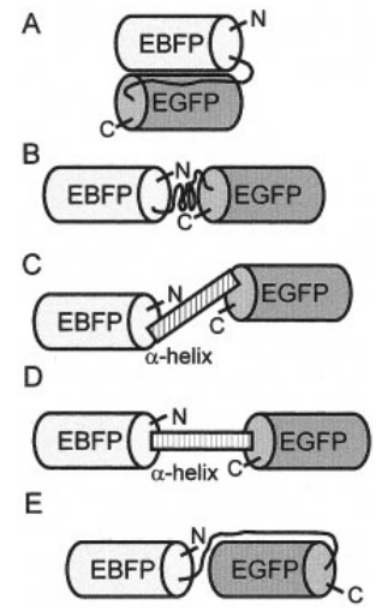
\includegraphics[width=0.3\textwidth]{img/conformacionLinker.png} 
\caption{Figura obtenida de \cite{arai2004conformations}}
\label{conformacionLinker}
\end{figure}


% como vimos antes, el proceso experimental asociado a obtener una proteína quimérica tiene varios pasos, y es importante que la etapa de diseño no se piense en la funcionalidad de la construccion(proteina) 
% de forma aislada sino que se tengan en cuenta las distintas técnicas que pueden/deben utilizarse durante el proceso y en los diferentes contextos donde la proteína se encontrará y donde deberá mantener sus propiedades.

El objetivo de la proteína es poder expresarla en un sistema biológico donde cumplira la función para la cual fue diseñada, por lo tanto es importante que las
propiedades conformacionales del linker se mantengan ante la presencia de otras proteínas o cualquier tipo de ligando.
% MOREs  y Agregacion




% Actividad biologica
La idea del diseño uniendo distintos módulos es que la funcionalidad global se origine exclusivamente a partir de la unión de éstos, por lo tanto la secuencia que los une no debe proveer ninguna funcionalidad adicional, es decir,
debe permanecer inerte ante el entorno en el cual la nueva proteína desarrolla su actividad. 
Las actividades biológicas pueden ser muy variadas pero   
Dado que las propiedades conformacionales  
Entre las actividades biológicas asociadas a estos segmentos están las modificaciones post-traduccionales, unión a ligandos, sitios de clivaje, etc.
Por lo tanto, es importante que la secuencia linker este libre de cualquier funcionalidad asociada a patrones secuenciales lineales. 






% 
% Los requerimientos en el linker no están limitados a la función o actividad de la proteína resultante. 
% Como se vió en la sección anterior, el proceso de 
% 


% COMPOSICION DE AMINOACIDOS: Carga metabolica y propiedades espectroscópicas
% Existen aspectos importantes a la hora de diseñar un linker que podrían parecer obvios, la composición y la longitud del linker son los primeros aspectos a considerar\cite{robinson1998optimizing}.



Por otro lado, la carga de la secuencia puede mediar interacciones en el entorno celular, por ejemplo, al construir proteínas cuya función requiera unirse al DNA es 
requerir que la secuencia linker no tenga residos carga ya que 

Otros requerimientos pueden no aparecer a partir de patrones secuenciales sino de propiedades intrínsecas de cada aminoácido. 
De esta forma, algunos requerimientos están relacionados con la composición secuencial. 
% CARGA METABOLICA
Un ejemplo claro de esto está en poder regular la carga metabólica asociada a la expresión de la secuencia linker. 
Dado que la proteína diseñada deberá ser, finalmente, expresada en algún sistema biológico, y que los distintos aminoácidos que conforman las proteínas tienen distintos costos metabólicos asociados, 
poder controlar la composición(imponiendo una menor frecuencia a aquellos aminoácidos con mas costo metabólico) permitiría incrementar el nivel expresión de la construcción creada.

% propiedades espectroscópicas
En otros casos, el requerimiento está asociado con propiedades fisicoquímicas de algunos aminoácidos. 
Por ejemplo, dado que las dado que las técnicas espectroscópicas se usan de forma rutinaria en el trabajo con proteínas, es deseable que el linker resultante tenga una composición específica tal que no posea aminoácidos que absorban en rango 
del UV, de forma que se elimine cualquier interferencia de la secuencia en este tipo de técnicas.

Otro ejemplo que afecta a la composición está asociada con interacciones iónicas no deseadas. 
Por ejemplo al construir una proteína cuya funcionalidad esté asociada a la unión a DNA, será deseable que la composición final no contenga aminoácidos que puedan encontrarse en estados con carga positiva, debido a que 
la formación de interacciones con la estructura de fosfatos propia del DNA podría interferir en la función de la proteína.

Teniendo en cuenta estos aspectos, una ventaja importante del proceso de diseño es poder definir la composición de la secuencia resultante.


% carga neta
% RESIDUOS CARGADOS
% Una ventaja importante del proceso de diseño es que se pueda definir la carga neta que tendrá la secuencia linker. 
% Este requerimiento puede tener varios fundamentos, principalmente 
Distintas técnicas de laboratorio para identificación y purificación de proteínas se basan en la carga neta de la secuencia.




% Esto se traduce en dos propiedades de la secuencia: que adopte una conformación extendida evitando que los dominios se compacten en el sitio de unión a través del linker, y que no posea una tendencia a adoptar estructuras secundarias, 
% ya que estas podrían reducir el número y tipo de interacciones posibles entre los dominios.


% Es relevante aclarar acá que, si bien los terminos desordenado y flexible pueden solaparse en algun punto, son términos distintos\cite{radivojac2004protein}
% Para una proteína plegada, la flexibilidad refiere a la desviación de las posiciones atómicas con respecto a la estructura promedio en equilibrio.
% Para una region desordenada, la variación en la flexibilidad se refiere a las diferencias en las velocidades de interconversión entre los diferentes estados miembro del ensamble estructural.
% Una variedad de técnicas biofísicas, como por ej. NMR, han sido usadas para estudiar estos conceptos de flexibilidad.

% Análisis de estructuras mediante estas tecnicas muestran que el movimiento en la proteína que provoca los cambios conformacionales puede ocurrir tanto a nivel de residuos como a nivel de estructura secundaria o terciaria. 


% Control of structural flexibility is essential for the proper functioning of a large number of proteins and multiprotein complexes. 
% At the residue level, such flexibility occurs due to local relaxation of peptide bond angles whose cumulative effect may result in large 
% changes in the secondary, tertiary or quaternary structures of protein molecules. 
% Such flexibility, and its absence, most often depends on the nature of interdomain linkages formed by oligopeptides.


% residues or at the secondary, tertiary, or quaternary structural levels. 
% Lactate dehydrogenase, triose-phosphate isomerase, as well as hemoglobin 
% and related proteins are some of the earliest examples of proteins that showed conformational changes with important functional implications.

% 



% 
% 
% 
% 
% La arquitectura típica creada, representada por dominios globulares unidos por secuencias linkers, busca que éstos permitan 
% mantener los dominios separados a la vez que se les da suficiente capacidad para moverse libremente como parte de su funcionalidad. 
% Por lo tanto, la flexibilidad es el requerimiento mas importante, y es deseable que un linker tenga tendencia intrínseca a adoptar una conformación extendida.
% Es importante que, como parte del diseño de la secuencia linker, se asegure que codifique una conformación intrínsecamente desordenada que no posea las características de una estructura colapsada propia de proteínas globulares.
% La conformación extendida le provee la flexibilidad global necesaria, a partir de la rápida interconversión entre la gran cantidad de conformaciones del ensamble con valores de energía similares.
% 
% 
% Un requerimiento asociado 
% Asociado a esto está la idea que una propiedad altamente desfavorable para el linker es que tenga cierta tendencia a adoptar estructuras de hojas-$\beta$ o helice-$\alpha$, ya que los angulos de torsion están limitados al rango
% impuesto por esta estructura, lo que podría también limitar la flexibilidad.
% Como vimos en las secciones previas, 
% aún cuando estas no se encuentren en una conformación plegada compacta típica de proteínas globulares.
% 



% SIGO CON EL EJEMPLO DE FRET QUE HAY MUCHA INFORMACION Y GRAFICOS INTERESANTES
% el ejemplo de FRET permite ejemplificar los requerimientos conformacionales, principalmente de flexibilidad. 
% En este caso, 
% Dado que, la funcionalidad resultante de la proteína quimérica creada depende completamente de la capacidad que 
% 







% % % % % % % ESTO LO PUEDO PASAR A LA PARTE DE LINKERS EMPIRICOS
% 
% % ACA EMPIEZO A HABLAR DE OTROS ASPECTOS NO ESTRUCTURALES
% Sin embargo, la flexibilidad no es todo.  
% Por ej. una opción evidente seria usar linkers de solo Glicina ¿Por qué no usar siempre un linker puramente poli-G, adaptando solamente su longitud?
% Desde los primeros estudios sobre linkers naturales \cite{argos1990investigation} se encontró que las proteinas naturales no usan(seleccionan) este tipo de secuencias.
% Si bien esto no es concluyente para que no se usen, puede darnos un motivo para pensarlo dos veces.
% En primer lugar, un péptido poli-G sería extremadamente inestable y por lo tanto podría actuar como una carga energética, estructural o interferir en procesos de catálisis de los dominios que une, 
% especialmente si tiene una longitud excesiva.
% Se conoce además que el patrón Gly-Gly-X, donde X es un residuo con cadena lateral hidrofóbica, es un sitio target de actividad proteolítica. 
% Por otro lado, una secuencia nucleotídica con alto contenido de Guanina(el codón que codifica para Glicina contiene Guanina en 2 de las 3 posiciones) puede ser difícil de manejar experimentalmente y de expresar para el huésped.
% Como se ve, entonces, existe una gran variedad de aspectos a considerar que exigen distintos requerimientos además de las propiedades conformacionales.
% Por ejemplo, es importante que los linkers should be invulnerable to host proteases, as they are often the targets for degradation. 
% 
% 
% El linker poli-G es sólo un ejemplo. 
% Como vimos en secciones anteriores, distintos elementos funcionales(que actuan principalmente mediante mecanismos de reconocimiento) pueden encontrarse en regiones con distintas propiedades conformacionales. 
% La existencia de estos elementos debe tenerse en cuenta cuando se esta usando la secuencia linker diseñada, y/o su eliminación debe formar parte de la etapa de diseño del linker.
% La longitud del \textit{loop} creado por el linker puede tener un profundo efecto sobre la actividad del linker en una proteína quimérica\cite{nagi1997inverse}.
% Además del ejemplo simple de resistencia proteolítica, las regiones linker también pueden afectar la estabilidad, solubilidad, formación de complejos.
% linker regions can affect the stability, solubility, oligomeric state, and proteolytic resistance ofthe fused protein
% Como se muestra en \cite{robinson1998optimizing}, en algunos casos se tienen efectos importantes variando la longitud y composición de la secuencia
% En base a esto, es esperable que se tengan requerimientos específicos relacionadas con la longitud y la composición. 
% % The stable linkage between functional domains provides many advantages such as a prolonged plasma half-life (e.g. albumin or Fc-fusions). 
% % However, it also has several potential drawbacks including steric hindrance between functional domains, decreased bioactivity, and altered biodistribution and metabolism of the protein moieties due to the interference between domains 
% % In other systems, however, linker regions can affect the stability, solubility, oligomeric state, and proteolytic resistance of the fused proteins
% % Thus, it is important that the length and amino acid composition of a potential linker is optimized in order to preserve the biological activity of the individual proteins in the fused complex.
% 
% 





% \subsubsection{Diseño negativo}




% Además de los analisis sobre las propiedades físicas asociadas a las arquitecturas modulares, el estudio de la diversidad de linkers
% encontrados en la naturaleza puede proveer información importante para entender los requerimientos
% más importantes en el diseño de estas secuencias.


\subsubsection{Linkers naturales}



% 


% El 'descubrimiento' de las regiones/secuencias linkers esta ligado a las teorias de structura-funcion(desarrolladas en la parte de conformacion) que se dieron durante casi 100 años
% En un principio se comenzo a pensar en una estructura rigida asociada a la proteina, luego se fueron revelendo propiedades dinamicas que le permitian cumplir la funcion. 
% Todo esto esta muy asociado a las tecnicas experimentales que se fueron desarrollando.

Como se dijo antes, la modularidad en proteínas naturales es algo muy común y existen muchisimos ejemplos de proteinas multidominio compuestas de dos o mas dominios funcionales unidas por linkers.
Estas secuencias linker sirven, principalmente para mantener unidos los distintos dominios, pero también proveen muchas otras funciones a la proteína como intervenir en las interacciones cooperativas 
entre los dominios o formar parte de la actividad biológoica de la proteína.

El primer estudio realizado sobre secuencias linkers \cite{argos1990investigation} registra la preferencia intrínseca por las conformaciones desplegadas.   
Sin embargo este estudio está bastante desactualizado y los resultados no son representativos ya que se realizó sobre un total de 51 linkers detectados manualmente a partir de 32 proteínas.
En \cite{george2002analysis} se encuentra un análisis más actual sobre un total de 638 proteínas multidominio,  a partir de las cuales se determinaron las regiones linkers(un total de 1280) y dominos utilizando un método automático.

% encuentran los análisis mas detallados donde se estudian las propiedades generales de secuencias linkers naturales

En \cite{chen2013fusion} se revisan los resultados obtenidos en ambos con respecto a diversas propiedades como son longitud, hidrofobicidad, enriquecimiento de ciertos aminoacidos y estructura secundaria adoptada.


% in general, preferable amino acids were polar uncharged or charged
% residues, which constitute approximately 50\% of naturally encoded amino acids. Both
% studies suggested that Pro, Thr, and Gln were the preferable amino acids for natural linkers.

% The preferred linker amino acids observed in the majority of
% the linker sets are Pro, Arg, Phe, Thr, Glu and Gln, in order
% of decreasing preference

Among them, Pro is a unique amino acid with a cyclic side chain which causes a very
restricted conformation [25]. The lack of amide hydrogen on Pro may prevent the formation
of hydrogen bonds with other amino acids, and therefore reduces the interaction between the
linkers and the protein domains.
As a result, the inclusion of Pro residues might increase the
stiffness and structural independence of the linkers.

Proline is unique among protein residues as
it is a cyclic imino acid with no amide hydrogen to donate in
hydrogen bonding. Therefore, it cannot fit into the regular
structure of either $\alpha$-helix or $\beta$-sheet and is a common ``breaker''
of secondary structure.
Proline will introduce some motion into a
helix, that enables a number of different conformations at that
region

Short proline rich sequences are
stiff, with non-interacting connections. As suggested before,
this is the most likely reason why proline is the preferred
linker constituent, particularly in non-helical linkers. It cannot
hydrogen bond to any surrounding amino acids, avoiding
ordered structure formation and contact with the neighbouring
domains.




% PROPIEDADS ESTRUCTURALES

% ESTRUCTURA SECUNDARIA
% Natural linkers adopt various conformations in secondary structure, such as helical, β-strand, coil/bend and turns, to exert their functions.
% the largest proportion of linker residues, 38.3\%,
% adopt the α-helical secondary structure, 13.6\% are in
% β-strands, 8.4\% are in turns and the rest, 37.6\%, are in coil
% or bend secondary structures.


En general, se encontro que los linkers naturales adoptaban principalmente conformaciones desplegadas y tenían estructuras independientes sin interacciones con los dominios adyacentes.
En términos de estructura, por ejemplo, se encontraron tanto linkers flexibles como relativamente rígidos en muchas proteínas.
A través de una mayor rigidez, ciertos linkers pueden ayudar a reducir interacciones no funcionales entre los dominios que unen. 
Por otro lado, una estructura más flexible, como es usual para conformaciones extendidas, provee una mayor flexibilidad y libertad de movimiento a los dominios.


% En \cite{george2002analysis} se esboza una clasificación de los linkers de acuerdo al análisis de su estructura secundaria.
% Se dividen, así, en dos categorías: helicoidales y no helicoidales.
% Los linkers con estructuras de $\alpha$-hélice pueden tener funciones como, por ejemplo, actuar como espaciadores rígidos impidiendo interacciones no funcionales entre los dominios.
% Aunque no sea exhaustiva, esta clasificación permite ver diferencias en los linkers también a nivel de estructura que adquieren, existiendo linkers que, a través de una mayor rigidez, impiden . 




Todas las propiedades analizadas(longitud, composición, hidrofobicidad y estructura secundaria.) resultaron importantes para alcanzar las funciones deseadas.


% AL FINAL DE TODO PONGO ESTOS EJEMPLOS, DEMOSTRANDO QUE LA FUNCIONALIDAD DE LOS LINKERS NO ESTÁ LIMITADA A PROVEER FLEXIBLIDAD Y QUE PUEDEN CUMPLIR OTRAS FUNCIONES

%EJEMPLOS DE PROPIEDADES CONFORMACIONALES
En terminos de flexibilidad, y por lo tanto de propiedades conformacionales en general, los linkers muestran 

en algunos casos la flexibilidad provista por los linkers naturales se origina a nivel de estructura secundaria, y esta limitada a una región corta que funciona como bisagra.
% EJEMPLO!!!!
En otros casos la flexibilidad es ``completa'' y la región del linker es intrínsecamente desordenada\cite{luo2010flexibility}, 
% EJEMPLO !
encontrándose incluso que la funcionalidad de la proteína se pierde cuando se reemplaza por un linker con \cite{hrycyna1998structural}

Ademas, existen linkers que, a pesar de mantener una conformación extendida en solución, pueden plegarse (o fijar una estructura secundaria transitiva) en presencia de ligandos.
Por ejemplo en el caso de ciertas proteínas que se unen a DNA\cite{laity2000dna}
%ESTE ES UN EJEMPLO DE FUNCIONALIDAD 


En algunos casos, las secuencias linker permiten mediar la propagacion eficiente de los efectos originados por la unión de ligandos o modificaciones post-traduccionales en uno de los dominios que conecta(alosterismo).
Un ejemplo es el caso de la miosina del musculo liso, en la cual un dominio que comprende la funcion motora es activado mediante fosforilacion  de una cadena regulatoria unida a este mediante un linker\cite{ikebe1998hinge}.
% OTRO EJEMPLO
% An example is the intramolecular interaction between the Src homology domains (SH2 and SH3) and the catalytic domains of Src family kinases, which results in repression of catalytic
% activity. Repression by the regulatory domain is nullified upon mutation of Trp260 to Ala within the linker separating the SH2 and kinase domain, which proves that the linker plays a crucial role in the coupling of
% the regulatory domains to the catalytic domain



%  ejemplo de la importancia de la secuencia linker en 
% otro ejemplo de funcionalidad esta en  \cite{tsutsumi2012charged}  ...



% CONCLUSIONES
Por lo tanto, a pesar que la flexibilidad es un aspecto que se sabe esta ligado a las secuencias linker en la naturaleza\cite{wriggers2005control}, 
y que estás regiones son generalmente las que permiten los grandes cambios conformacionales en las estructuras de las proteínas, 
estas no son simplemente secuencias que evolucionan hacia conformaciones totalmente flexibles, ya que esto puede no estar directamente ligado al cumplimiento de la función requerida, o no hacerlo de forma eficiente.

De esta forma, las secuencias linker en la naturaleza son una parte mas de las proteínas y sus propiedades conformacionales no pueden definirse como generales, sino que están 
% De esta forma, las propiedades conformacionales de las regiones linkers naturales están usualmente 
asociadas a restricciones funcionales de la proteína global, buscando balancear la flexibilidad requerida 
para que los dominios puedan explorar el ensamble de conformaciones asociado a su funcionalidad, con la rigidez requerida para que no existan interacciones desfavorables entre estos, 
resultando en perfiles muy variados de flexibilidad.

En cada proteina, la secuencia linker puede tener una estructura y una función que haya sido seleccionada para el mecanismo/localización/función de la proteina como un todo, 
y esta función del linker puede no ser solamente la unión covalente de dos dominios. 

Las propiedades funcionales no solo afectan a la conformación sino que abarcan la longitud, composición y propiedades secuenciales puntuales.





% UTILIZACION DE LINKERS NATURALES PARA 
Dado este contexto, el uso de secuencias linkers naturales en el contexto del diesño de proteínas quiméricas debe realizarse con mucho cuidado.
........

% ACÁ PUEDO PONER QUE LOS LINKERS NATURALES TAMBIEN PUEDEN SERVIR COMO BASE PARA UN PROCESO DE INGENIERIA?? O LO PASO A LA PROX. SECCION???









% Los primeros estudios de analisis (estructura y composicion) de secuencias linkers\cite{argos1990investigation} se comenzaron a hacer a partir del analisis estadistico de secuencias que podian ser clasificadas 
% como linkers a partir de las primeras estructuras de proteinas multidominio almacenadas en bases de datos.
% % Estos estudios estaban sesgados por todo el proceso historico de descubrimiento marcado por 
% Los resultados indicaban que la mayoria adquiría una conformación desplegada(tipo \textit{coil}) sin estructura secundaria. 
% % many studies of linker peptides in various protein families have come to the conclusion that linkers lack regular secondary structure (la mayoria se encontraba en estructuraas tipo coil), 
% % they display varying degrees of flexibility to match their particular biological purpose and are rich in Ala, Pro and charged residues
% Asi surgio la idea que los linkers eran secuencias cortas cuya unica funcion era proveer la conexion covalente, lo que estaba de acuerdo con el concepto de hinge-bending.
% Este concepto indicaba que la flexibilidad de estas regiones cortas dentro de un polipéptido permitía el suficiente movimiento a los dominios estructurales.
% % The concept of hinge-bending, whereby the relative flexibility of these short regions of the polypeptide chain allows significant movement of structural domains, gained widespread acceptance in
% % the 1980s and early 1990s, after evidence for conformational transitions in identical or homologous proteins became known.



% A lo largo de los años los conocimientos sobre la composición y propiedades de estas secuencias ha ido cambiando, 
% a medida que mayor cantidad de estructuras se resolvian y mayor conocimiento se obtenia acerca de los dominios que componen 
% las proteinas. Tambien influyeron otras cosas como tecnicas biofisicas que permiten obtener información del ensamble conformacional en solución,
% o algoritmos para automatizar la identificación de los dominios y las secuencias que actúan como linker en una proteina.
% 

% Although the role of linker sequences is likely to be primarily topological, allowing distant parts of the polypeptide chain to interact with diverse partner sequences that might be far apart or close together, 
% linkers and unstructured tail sequences play quite specific roles in a number of systems.








% A FUTURO
Con el incremento del número de estructuras almacenadas en la PDB que ocurrió en los últimos años, sería posible realizar un estudio actualizado de las propiedades de los linkers naturales.
Además, sería interesante extender el número de propiedades analizadas agregando categorías asociadas a función y estructura de la proteína, e identificando la relación entre estas y las propiedades del linker.
% With the rapid increase of the number of protein structures deposited in the PDB database, an updated study of natural linkers could be conducted. 
% In addition to the properties analyzed in previous studies (e.g., amino acid composition, structure classification), 
% it would be interesting to categorize the multi-domain proteins by their functions and structures, and identify the relationship between them and the linker properties


% 
% 
% Based on From George and
% Heringa’s secondary structure analysis, linkers were grouped into two categories: helical and
% non-helical. The $\alpha$-helix was a rigid and stable structure, with intra-segment hydrogen bonds
% and a closely packed backbone [28]. Some $\alpha$-helical conformations form rapidly during
% folding [28], allowing the correct folding of connecting protein domains without non-native
% interactions with the linker. Linkers in an $\alpha$-helix structure might also serve as rigid spacers
% to effectively separate protein domains, and to reduce their unfavorable interactions.
% Therefore, this conformation was commonly adopted by many natural and empirical linkers
% (to be discussed later). On the other hand, without an inherent rigid structure, the non-helical
% linkers tended to be rich in Pro, which could increase the stiffness of the linker as mentioned
% previously [25]. As a result, non-helical linkers with Pro-rich sequence could exhibit
% relatively rigid structures and serve to reduce inter-domain interference.
% 
% 
% 
% Both flexible and relatively rigid peptide linkers are found in many multidomain proteins. 
% Linkers are thought to control favorable and unfavorable interactions between adjacent domains by means of variable softness
% furnished by their primary sequence. Large-scale structural heterogeneity of multidomain proteins
% and their complexes, facilitated by soft peptide linkers, is now seen as the norm rather than the
% exception. Biophysical discoveries as well as computational algorithms and databases have
% reshaped our understanding of the often spectacular biomolecular dynamics enabled by soft linkers.
% Absence of such motion, as in so-called molecular rulers, also has desirable functional effects in
% protein architecture.







% 
% 
% \subsubsection{Molecular rulers}
% These linkers are more defined by their ability to reliably predict and maintain end-to-end distances between attached domains. 
% Such structurally rigid peptides have been conjugated to molecules to serve a metric function.
% These linkers are rich in Proline. 
% Proline is common to many naturally derived interdomain linkers, and structural studies indicate that proline-rich sequences form relatively rigid extended structures to prevent unfavorable interactions between the domains.
% The probable reason why proline is favored over other residues in linking different domains is the inability of proline to donate hydrogen bonds or participate comfortably in any regular secondary structure conformation. This ensures a relatively rigid separation of the domains, thereby preventing unfavorable contacts between them.
% 
% Although short stretches of hard linker sequences are located between functionally relevant regions of protein structure, mutations within such sequences may have no effect on the function.  
% Such linkers are therefore necessary to keep the other amino acid interactions in register, but the nature of the side chain is often unimportant.
% 
% The observed natural tendency to form rigid linkers might also
% be related to avoiding proteolytic cleavage, as linkers are likely
% targets for protease degradation
% 
% Linker
% sequences vary greatly in length and composition, but
% many are rich in polar, uncharged amino acids (such as
% Ser, Thr, Gln and Asn), in the small residues Ala and Gly,
% and in Pro residues. Many of these residues tend to bias
% the polypeptide chain towards the polyproline-II region
% of the RAMACHANDRAN PLOT 27,28 .This means that such
% linkers, although flexible, have a propensity to be highly
% extended. Compositionally biased linker sequences of
% significant length are found mainly in eukaryotic pro-
% teins 1,29 , but short linker sequences of similar composi-
% tion, known as Q-linkers, are also found in a number of
% bacterial regulatory proteins 30 .
% In the absence of their targets, modular proteins
% often behave as ‘beads on a flexible string’, where the
% function of the linker is, primarily, to enable a relatively
% unhindered spatial search by the attached domains 31 .
% However, binding can induce structure formation in
% linkers, which can have significant functional conse-
% quences. For example, the sequence-specific binding of
% CYS HIS ZINC-FINGER PROTEINS to DNA causes the linker to
% fold, cap and thereby stabilize the preceding helix in the
% protein, and to orientate the next zinc finger correctly
% for binding in the major groove of DNA
% 
% 















\subsubsection{Diseño racional}


Con tantos, y tan distintos, requerimientos positivos y negativos, el problema del diseño de linkers puede llegar a ser un tema complejo.
El problema del diseño racional es, entonces, un proceso complicado.
% The general properties of linkers derived from naturally-occurring multi-domain proteins(que se vieron en la seccion anterior) can be considered as the foundation in linker design. 
Las propiedades generales de los linkers naturales encontrados en proteínas multi-dominio pueden considerarse como un primer paso hacia el proceso de diseño.



% PRIMERO HABLAR DE LINKERS USADOS EMPIRICAMENTE 

% Además de la utilización de linkers naturales, una opción común es reutilizar linkers ya utilizados empíricamente, 
La opciones actuales del diseño de linkers se basan, generalmente,  en reutilizar secuencias ya evaluadas empíricamente, buscando la que más se adapte a nuestros requerimientos. 
Muchas de estas secuencias son linkers naturales y otros han sido modificados especificamente en cada caso por procesos de ingeniria.
% Linker engineering, with the aim to control the distance, orientation, and relative motion of two functional domains, will increase in importance with increasing emphasis on the de novo design of multi-domain proteins.
En \cite{chen2013fusion} se hace un análisis de los linkers empíricos más usados para creación de proteínas quiméricas y que pueden encontrarse en literatura, diseñados mediante aproximaciones muy distintas.
A partir de esta recopilación se intenta hacer una clasificación general que resulta en 3 categorias:
linkers flexibles, linkers rígidos, y linkers que pueden experimentar clivaje \textit{in-vivo}. 
Como se puede ver, esta clasificación esta basada, principalmente, en propiedades estructurales/conformacionales. 
Para obtener secuencias que posean otras propiedades de interés deberán analizarse cada uno de los linkers que se detallan en este trabajo.
Los linkers que se encuentran  en la literatura fueron construidos en base a la intuición y la posterior validación experimental.


En el caso de fusiones que requieren linkers flexibles, la mayoría se construye en en base a la intuición utilizando residuos pequeños(polares o no polares) tales como Gly, Ser y Thr,
siendo el linker más común encontrado en la literatura el compuesto por distinto número de repeticiones del motivo $(G_4S_n)$. %PONER REFERENCIAS AL USO DE ESTE.
También se ha utilizado linkers poliglicina($G_n$), en estos casos la sustitución de algunas posiciones por residuos polares (Ser) busca reducir las interacciones no deseadas entre el linker y los dominios que une de forma
tal que no interfieran en la funcionalidad.
Una aproximación de diseño más avanzada se puede ver en \cite{bird1988single}, donde se utilizan residuos Gly y Ser para proveer flexibilidad pero se agregan Glu y Lys para incrementar la solubilidad.
% COMENTAR EL METODO USADO MAS EN DETALLE


% peptide sequences consisting of flexible and hydrophilic residues (arbitrary repeats of glycine and serine residues) are used because they are assumed to form a random coil and do not interact with (the folding of)
% the protein domains
En la mayoría de estos casos, los péptidos con motivos repetidos de Gly y Ser son usados porque se asume que adoptan una conformacion similar a random coil y no interfieren en el plegado y funcionamiento de los dominios que unen,
la funcionalidad provista por estos se evalúa en cada caso en particular.
En \cite{evers2006quantitative} se hace una evaluación de estos linkers tan usados, en el contexto de la unión de dos proteínas fluorescentes, evaluando cuantitativamente las propiedades conformacionales y el efecto de la longitud del linker 
a partir de la transferencia de energía entre estas.


Estos linkers poseen conformaciones desestructuradas (Gly suele considerarse como capaz de romper la estructura ordenada de las hélices), y esta flexibilidad puede, en algunos casos, impedir que se logre una separación 
suficiente entre los dominios (Evers et al., 2006).

As a result, more rigid linkers including polyproline motifs (
Schuler et al., 2005 ) and an all
a-helical linker A(EAAAK)n A(Arai
et al ., 2001) have been developed.




% LINKERS RIGIDOS
% ref 34 = \cite{arai2001design}
% ref 35 = \cite{arai2004conformations}
% 
% An empirical rigid linker with the sequence of A(EAAAK) n A (n = 2-5) was first designed
% by Arai et al. [34, 35]. The linker displayed α-helical conformation, which was stabilized by
% the Glu − -Lys + salt bridges within segments. To test whether they could effectively separate
% the protein domains, these helical linkers were inserted between enhanced blue fluorescent
% protein (EBFP) and enhanced green fluorescent protein (EGFP), and the fluorescent
% resonance energy transfer (FRET) efficiency between EBFP and EGFP was measured [34].
% The FRET efficiency decreased as the length of helical peptides increased, indicating that
% helical linkers can control the distance between domains by changing repetitions of the
% EAAAK motif. Compared to flexible linkers with the same length, the helical linkers
% induced much less FRET efficiency when inserted into EBFP-EGFP fusion proteins,
% suggesting that helical linkers can separate functional domains more effectively.







% PONER LOS EJEMPLOS QUE USAN UNA COMBINACION DE ESTOS LINKERS RIGIDOS Y FLEXIBLES PARA UN DISEÑO DE FRET:
% el linker totalmente flexible permite todo tipo de interacciones entre los dominios, pero
% en este caso lo que se busca es que en la conformacion normal se evite lo mas que se pueda las interacciones entre dominios, ya que estas generan resonancia energetica no deseada(solo se quiere).
% primero: Antibody Detection by Using a FRET-Based Protein Conformational Switch: 
% aca lo que buscan es un linker suficientemente flexible para permitir la interaccion de las dos partes del sensor en su forma no unida al anticuerpo(teniendo asi una alta tasa de emision),
% pero que a la vez permita un 'efficient bridging'(mantenga cierta distancia) como para que, al unirse ambos extremos al anticuerpo, se pierda la interaccion disminuyendo la tasa de emision.
% primero usan un linker super flexible (17 Gly-SerGly repeat), despues prueban uno que incorpora motivos alfa-helice
% El segundo caso donde se usa este nuevo linker es en: a sensor for quantification of macromolecular crowding in living cells
% El linker que terminan usando en ambos es $A(EAAAK)_6A(GSG)_6A(EAAAK)_6A$








% DESPUES EMPIEZO CON DISEÑO RACIONAL

El diseño racional de linkers, sin embargo, está aún en los principios del desarrollo. 


% Although many examples of various types of linkers have been developed in the past, the rational design of linkers for the construction of fusion proteins is still in its infancy. 

En algunos casos se ha 
Existen pocos ejemplos concretos donde se haya utilizado una aproximación racional para el diseño de linkers \cite{arai2001design,arai2004conformations}.

Los estudios detallados de la composición, estructura y función de linkers naturales son un claro punto de inicio.
Con el rápido incremento de los conocimientos sobre la secuencia y estructuras de proteínas, nuevos estudios podrían aportar conocimientos relevantes en esta dirección.
Sin embargo no hay indicios sobre posibles desarrollos orientados a obtener un método sistemático para el diseño racional.  
% Systematic, strategic scientific endeavors are in demand to greatly advance the science of linker design and application.
% Many technology platforms may be investigated in more depth towards understanding the connection between linker composition and structure, and ultimately tie them to linker function.
% The study of linker composition and structure, and the investigation of linker function should go hand in hand when designing a novel linker.
% With the rapid increase of the number of protein structures deposited in the PDB database, an updated study of natural linkers could be conducted.
% The establishment of more databases and searching programs for linkers would be another fruitful direction. 
% As discussed earlier, only two studies have been performed to analyze the characteristics of the linkers in natural multi-domain proteins.
% ESTO ESTA CASI IGUAL EN LA SECCION ANTERIOR

% The extensive studies on the structures of empirical linkers have provided us with useful information for optimal linker design. 
% Ultimately, more searching algorithms for linker databases could be developed, and provide more linker candidates for protein fusion based on user specifications.










% FINALMENTE EXPLICAR LAS APROXIMACIONES RACIONALES QUE ENCONTRE, QUE CONSISTEN BASICAMENTE EN BUSCAR EN BBDD


Los estudios realizados sobre linkers naturales(mencionados en la sección anterior) abrieron la posibilidad de crear bases de datos conteniendo las secuencias encontradas y sus propiedades asociadas.
Asociados a estas bases de datos, se han desarrollado distintos métodos que permiten extraer  ,  que simula un mecanismo de diseño.
% The extensive studies about linkers in natural multi-domain proteins and recombinant fusion proteins fostered the idea of building databases and coming up with linker (designing??) tools 
% to aid the (rational???) design of linkers based on the desired characteristics of fusion proteins.
% Es decir, actualmente la metodologia esta centrada en crear bases de datos de linkers y hacer consultas sobre esta en base a las propiedades que se buscan.

Los resultados del estudio desarrollado en \cite{george2002analysis} son el primer ejemplo de este tipo de metodologías.
% An example of this type of tools was developed during the analysis of a protein dataset to obtain information about linker sequences 
En este trabajo se estudian diversos aspectos asociados a los linkers y se desarrolla una base de datos asociada a un algoritmo de búsqueda que puede ser utilizado mediante un servidor web\cite{linkerdbIBIVU}.
El algoritmo implementado acepta distintos parámetros de búsqueda tales como longitud del linker, accesibilidad del solvente, estructura secundaria adoptada, similitud secuencial con una secuencia input, etc.
% The search algorithm accepts several query types (eg, PDB code, PDB header, linker length, C-alpha extent, solvent accessibility, secondary structure or sequence). 
El programa devuelve las secuencias linker que contienen los criterios solicitados y, además, provee información del contexto en el que se encuentra el linker, con información del ID en PDB, descripciones de la proteína, etc. 
de forma que el usuario pueda inferir otras propiedades del linker que no pueden ser extraídas automáticamente.
% The program can provide the linkers sequences meeting the searching criteria, and also provide other information such as the PDB code and a brief description of the source protein, 
% linker’s position within the source protein, linker length, solvent accessibility, and secondary structure. 
% Users can search for sequences with desired properties, and obtain candidate sequences from natural multi-domain proteins.

Otro ejemplo de búsqueda sobre bases de datos es \url{http://bioinf.modares.ac.ir/software/linda/}

Un ejemplo más reciente de este tipo de aproximación mediante bases de datos da origen a la herramienta LINKER \cite{crasto2000linker,xue2004linker}.
% A more recent example of this type of tool is a program called LINKER 
Al margen de la falta de creatividad en el nombre de la aplicación, esta posee un método de búsqueda que brinda una gran cantidad de opciones al usuario incluyendo aspectos experimentales como la sensibilidad a la actividad de proteasas.
% which searches its database of linker sequences with user-specified inputs (e.g., linker length, protease sensitive sequences to be avoided), and generates an output of several linker sequences that fit the criteria.
En este caso, el centro del método es base de datos conteniendo secuencias loop extraidas de PDB y que son luego levemente procesadas removiento secuencias idénticas, hairpin loops y secuencias de menos de 4 residuos. 
El programa de búsqueda/diseño construido sobre esta base de datos asume que la conformación de loop adoptada por la estructura cristalizada que se encuentra en la PDB dará una conformación extendida 
si se utiliza esta secuencia como linker en una proteína quimérica
Desafortunadamente, el servidor web asociado a este programa no está más disponible.



Una nueva versión de este tipo de soluciones se realizó este año en \cite{liu2015synlinker}. 
La particularidad de esta nuevo programa es que incorpora en su base de datos, no sólo a secuencias linker naturales sino también algunos linkers empíricos extraídos de la literatura, 
que siguen los principios de diseño/construcción que vimos hasta ahora en esta sección.
Una particularidad de esta herramienta es que permite obtener un modelo computacional donde 1 o mas linkers se fusional con estructuras/dominios obtenidos de la pdb. 
Este modelo puede ser usado directamente como input en el próximo paso(siguiendo el esquema de la figura \ref{esquemaProcesoFusion}) donde se pueden evaluar mediante simulaciones de dinámica molecular algunas propiedades conformacioneles de la construccion obtenida.



A pesar que las bases de datos no proveen una solución total al problema de diseño, la construcción de estas y los métodos de búsqueda asociados 
ayuda a la utilización de los conocimientos adquiridos a partir de estudios sobre secuencias naturales.
% building an empirical linker database could help summarize the knowledge and facilitate the future linker design.
% The extensive studies on the structures of empirical linkers have provided us with useful information for optimal linker design. 
El desarrollo de métodos de búsqueda más abarcativos junto con nuevos estudios para encontrar secuencias linker naturales podría generar un avance en este tipo de metodologías.
% Ultimately, more searching algorithms for linker databases could be developed, and provide more linker candidates for protein fusion based on user specifications.
% Lo bueno de las BBDD es que los elementos que contienen suelen haber sido probados experimentalmente, lo cual es fundamental.








































% In summary, linkers can adopt various structures and exert diverse functions to fulfill the  application of fusion proteins (Table 2). 
% The flexible linkers are often rich in small or hydrophilic amino acids such as Gly or Ser to provide the structural flexibility and have  been applied to connect functional domains that favor interdomain interactions or
% movements. In cases where sufficient separation of protein domains is required, rigid linkers may be preferable. 
% By adopting α-helical structures or incorporating Pro, the rigid linkers can efficiently keep protein moieties at a distance. 
% Both flexible and rigid linkers are stable in vivo, and do not allow the separation of joined proteins. Cleavable linkers, on the other
% hand, permit the release of free functional domain in vivo via reduction or proteolytic cleavage. They can be utilized to improve the bioactivity of chimeric proteins, or to  specifically deliver prodrugs to target sites where the linkers are processed to activate bioactivity. The rational choice of linkers should be based on the properties of the linkers
% and the desired fusion proteins.

% 
% % FLEXIBLE LINKERS
% Flexible linkers are usually applied when the joined domains require a certain degree of movement or interaction. They are generally composed of small, non-polar (e.g. Gly) or polar (e.g. Ser or Thr) amino acids
% Este tipo de polipeptidos do not affect the function of the individual proteins to which they attach. 
% 
% The small size of these amino acids provides flexibility, and allows for mobility of the connecting functional domains. 
% The incorporation of Ser or Thr can maintain the stability of the linker in aqueous solutions by forming hydrogen bonds with the water molecules, and therefore reduces the unfavorable interaction between the linker and the protein moieties.
% The most commonly used flexible linkers have sequences consisting primarily of stretches of Gly and Ser residues (“GS” linker). 
% By adjusting the copy number “n”, the length of this GS linker can be optimized to achieve appropriate separation of the functional domains, or to maintain necessary inter-domain interactions.
% The loop length created by the linker can have a profound effect on the action of the linker in the fused complex
% 
% Many other flexible linkers have been designed for recombinant fusion proteins. As suggested by Argos [23], these flexible linkers are also rich in small or polar amino acids such as Gly and Ser, but can contain additional amino acids such as Thr and Ala to maintain flexibility, as
% well as polar amino acids such as Lys and Glu to improve solubility.
% 
% 
% 
% % LINKERS RIGIDOS (MOLECULAR RULERS)
% While flexible linkers have the advantage to connect the functional domains passively and
% permitting certain degree of movements, the lack of rigidity of these linkers can be a
% limitation. There are several examples in the literature where the use of flexible linkers
% resulted in poor expression yields or loss of biological activity.
% 
% The ineffectiveness of flexible linkers in these
% instances was attributed to an inefficient separation of the protein domains or insufficient
% reduction of their interference with each other. Under these situations, rigid linkers have
% been successfully applied to keep a fixed distance between the domains and to maintain their
% independent functions
% 
% The major concern in the design of a molecular ruler is the possibility of softening and structural failure that arises when the ruler is unable to provide a predictable separation distance between its bound
% moieties. An adequate cushion distance is often required when designing the linkers.
% 
% Alpha helix-forming linkers with the sequence of (EAAAK) n have been applied to the
% construction of many recombinant fusion proteins [18, 20]. As suggested by George and
% Heringa [24], many natural linkers exhibited $\alpha$-helical structures. The $\alpha$-helical structure
% was rigid and stable, with intra-segment hydrogen bonds and a closely packed backbone
% [28]. Therefore, the stiff $\alpha$-helical linkers may act as rigid spacers between protein domains.
% 
% 
% Another type of rigid linkers has a Pro-rich sequence, (XP) n , with X designating any amino
% acid, preferably Ala, Lys, or Glu. As suggested by George and Heringa [24], the presence of
% Pro in non-helical linkers can increase the stiffness, and allows for effective separation of
% the protein domains. The structure of proline-rich sequences was extensively investigated by
% several groups
% 
% Un ejemplo interesante, relacionado con la aplicacion que motivó este trabajo(FRET) se puede ver en (ref Design of the linkers which effectively separate domains of a bifunctional fusion protein - Ryoichi Arai,): 
% En este trabajo.....
% An empirical rigid linker with the sequence of A(EAAAK) n A (n = 2-5) was first designed.
% The linker displayed  $\alpha$-helical conformation, which was stabilized by
% the Glu Lys salt bridges within segments. To test whether they could effectively separate
% the protein domains, these helical linkers were inserted between enhanced blue fluorescent
% protein (EBFP) and enhanced green fluorescent protein (EGFP), and the fluorescent
% resonance energy transfer (FRET) efficiency between EBFP and EGFP was measured [34].
% The FRET efficiency decreased as the length of helical peptides increased, indicating that
% helical linkers can control the distance between domains by changing repetitions of the
% EAAAK motif. Compared to flexible linkers with the same length, the helical linkers
% induced much less FRET efficiency when inserted into EBFP-EGFP fusion proteins,
% suggesting that helical linkers can separate functional domains more effectively.
% 
% 
% % IN-VIVO CLEAVABLE LINKERS
% Under these circumstances, cleavable linkers are introduced to release free functional
% domains in vivo . The design of in vivo cleavable linker in recombinant fusion proteins is
% quite challenging. Unlike the versatility of crosslinking agents available for chemical
% conjugation methods, linkers in recombinant fusion proteins are required to be
% oligopeptides. The linkers introduced in this section take advantage of the unique in vivo
% processes, and are cleaved under specific conditions such as the presence of reducing
% reagents or proteases. This type of linker may reduce steric hindrance, improve bioactivity,
% or achieve independent actions/metabolism of individual domains of recombinant fusion
% proteins after linker cleavage
% 



       
       
       
       
       
\section{Objetivos}

El objetivo principal de este trabajo es implementar un método para generar una secuencia linker \textit{de novo} a partir de los requerimientos descritos, o adaptando una secuencia inicial provista por el usuario a estos requerimientos. 
Como requerimientos fundamentales de la secuencia resultantes deberán cumplirse que la misma provea la flexibilidad necesaria para cumplir su función como linker en la creación de nuevas proteínas quiméricas.
Además, esta debe mantenerse inerte frente a cualquier actividad que pueda interferir durante el proceso experimental asociado o en el correcto funcionamiento del diseño final.
% La herramienta buscará proveer, además, diversas utilidades que servirán para que el resultado obtenido sea lo mas adecuado posible para su uso experimental. 	

%     (esquema muy simplificado del input/output del algoritmo)
% HACER GRAFICO          INPUT --- PROCESO ---->> OUTPUT    
%            INPUT: preferencias del usuario(longitud o secuencia inicial, composicion, carga neta, silente en UV)  ------->>   
%            PROCESO OCULTO AL USUARIO: a partir de la secuencia inicial o una secuencia random con la longitud iniciada se eliminan las propiedades
% 					conformacionales y funcionales no deseadas, llevando a una secuencia final con propiedades flexible, sin elementos funcionales y acorde a los requerimientos indicados por el usuario   -------->>>   
%             SALIDA: secuencia acorde a los requerimientos del usuario y propiedades de un linker flexible

El esquema de la herramienta resultante se muestra, de forma simplificada, en la figura \ref{diagram}

% https://www.draw.io/
\begin{figure}[h!]
\centering
   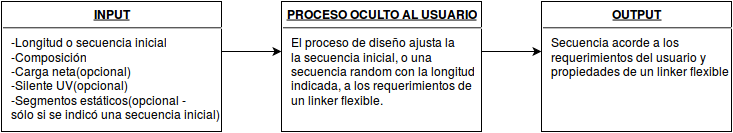
\includegraphics[width=\textwidth]{img/diagram.png}
 \caption{Esquema general de la herramienta implementada}
 \label{diagram}
\end{figure}

